\chapter{相关工作}\label{chap:relate}

本章的主要内容分为三个部分,第一部分主要介绍微表情研究中使用的数据集以及微表情和常见的宏表情之间的差异,第二部分介绍近几年微表情研究中所使用的特征提取的几种方法,
第三部分介绍本文将在第四章中使用的相关深度网络的基础知识。

\section{宏表情和微表情}

普通的人脸表情可以是自然产生的,也可以是根据需要人为的摆拍出来。摆拍的人脸表情是有意表现出某种情绪,而自然产生的人脸表情是在表达自己的真实情感。所以在人脸宏表情
(普通人脸表情)的研究中,既有自然产生的表情数据,也有摆拍的表情数据,微表情研究也存在类似的问题。在微表情研究领域用“自发”这个词来强调微表情的产生(或被诱导)是自
然的,因为参与者的内心存在实际的情感。

所以根据表情的产生方式将微表情分为“自发”产生的真实微表情和“摆拍”的微表情。目前摆拍的数据集主要有USF-HD数据集和Polikovsky数据集,自然状态下诱发产生的自发数据集,
主要包括SMIC、SMIC2、CASME、CASME II和SAMM等数据集,本节将简单介绍几种数据集的产生方式和优缺点,同时列举典型的宏表情数据集做对比,明确微表情的概念。。

\subsection{宏表情数据集}

随着图像识别和表情研究的深入,宏表情数据集的建立越来越完备。目前常用的人脸宏表情数据集有日本女性表情库(The Japanese female facial expression,JAFFE)\citep{Lyons2002Coding}、Yale表情数据集\citep{Belhumeur2002Eigenfaces}和CK+人脸表情数据集\citep{Lucey2010The}等。本文提出的算法中没有用到宏表情,此处以最常用的CK+数据集举例只为说明宏表情和微表情之间的差异。

CK+数据集是在Cohn-Kanade Dataset的基础上扩展来的,发布于2010年。2000年,Cohn-Kanade(CK)数据集发布,目的是促进人脸面部表情的自动检测研究。从那时起,CK数据集成为算法开发和评估中使用最广泛的测试平台之一。在此期间,产生了三个明显的局限性:1)虽然AU编码经过了很好的验证,但是情感标签是错误的,因为标定的标签是被要求的,而不是实际产生的;2)对新算法的评估缺乏一个通用的性能指标;3)不包含常见数据集的标准协议。因此,CK数据集被用于AU和情感检测时缺少与基准算法的比较,并且使用原始数据集的随机子集使得对元数据的分析变得困难。为了解决这些问题,发布了扩展版的Cohn-Kanade数据集CK+。CK+数据集中的表情分为三类,包括了摆拍和自发的表情以及其他类型的元数据(Metadata)。对于摆拍的表情,序列的数量比第一版的增加了22\%,参与者的数量增加了27\%。与初始版本一样,每个序列的目标表情都是完整的FACS编码,情感标签也经过了修改和验证。此外,元数据中还添加了经过验证的情感标签。数据集中还包含使用主动外观模型(Active Appearance Models,AAMs)和线性支持向量机分类器给出的基线结果,使用留一法交叉验证对摆拍的数据进行AU和情绪检测。

CK+数据集包括123个参与者,593个图像序列,每个图像序列的最后一张帧有AU标签,而在这593个图像序列中,有327个序列有情感标签。CK+数据集是人脸表情识别中比较流行的一个数据集,该数据集将情感分为8类,包括中性,厌恶,愤怒,蔑视,压抑,快乐,悲伤,惊讶。图~\ref{fig1}给出了该数据集中的样本图片。综合来说,CK+是目前较为理想的表情数据集。

\begin{figure}[!htbp]
    \centering
    \begin{subfigure}[b]{0.22\textwidth}
      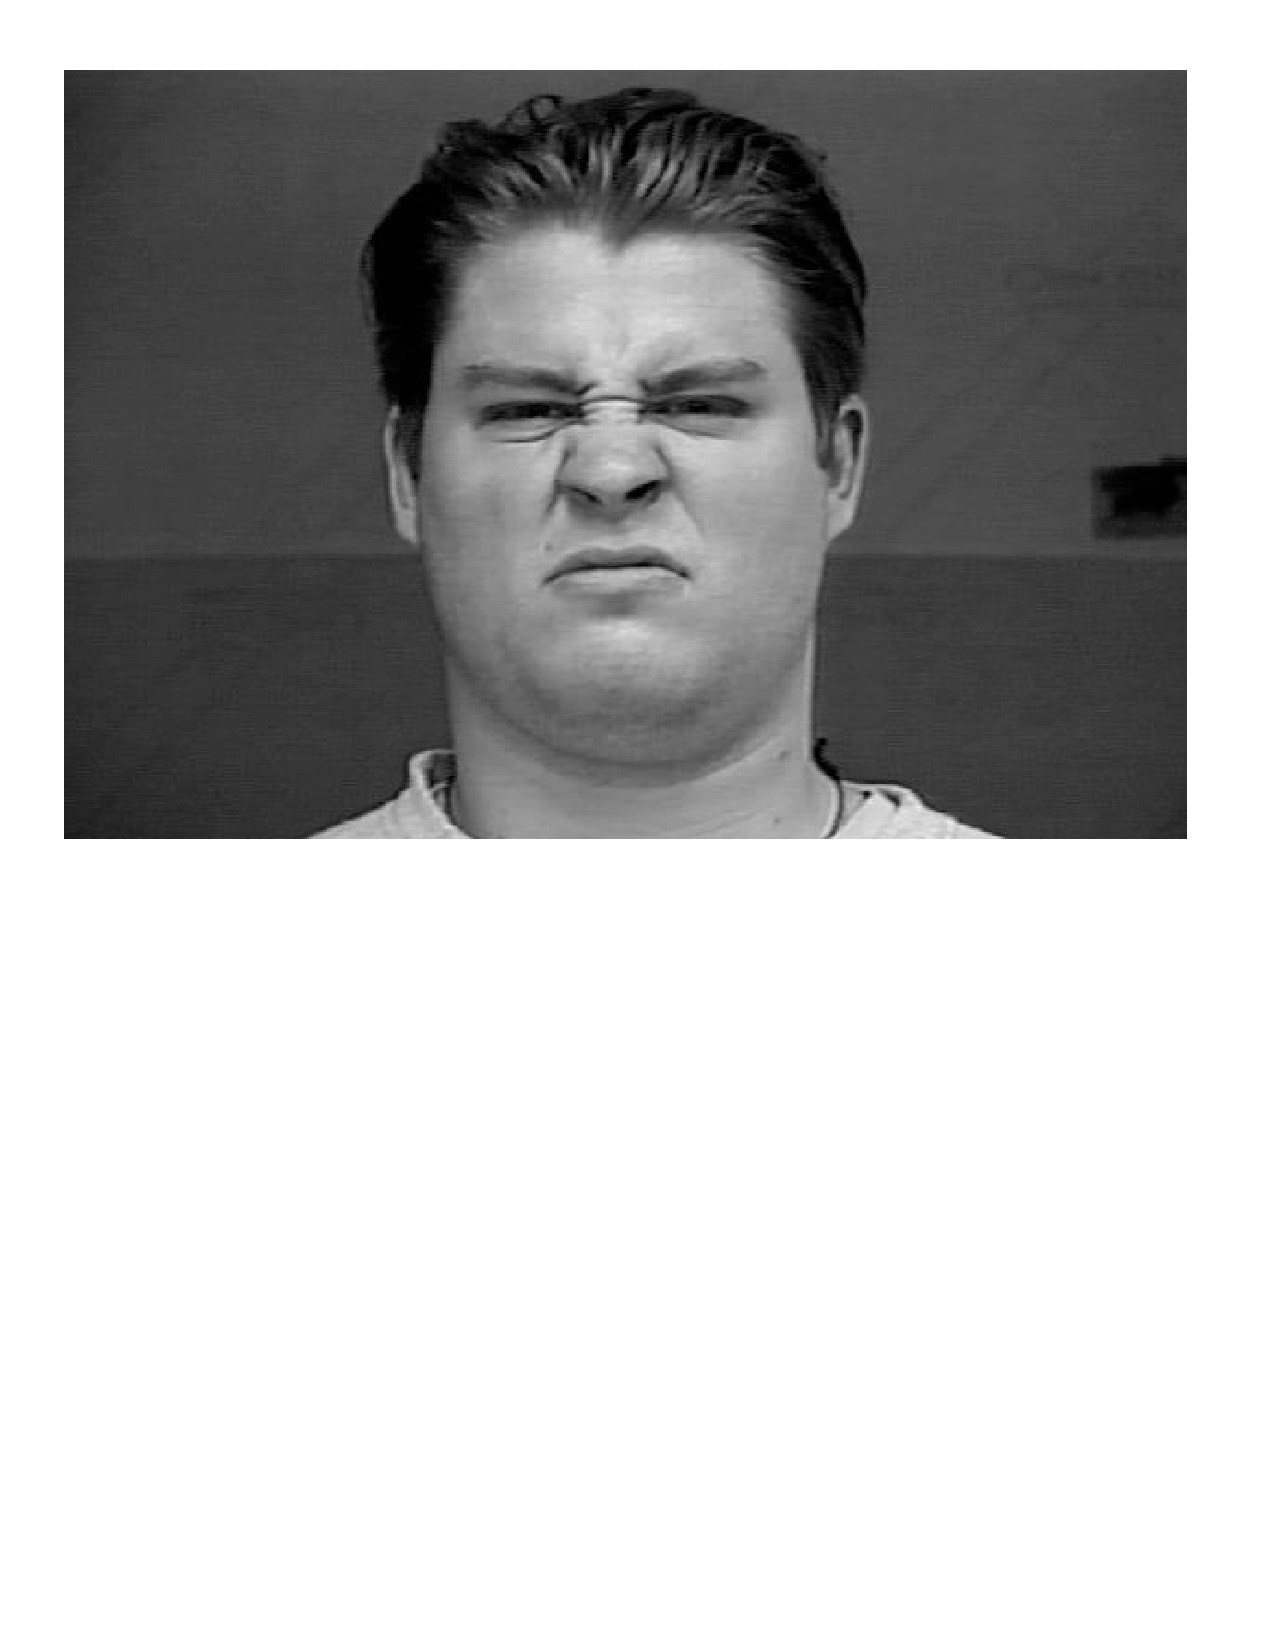
\includegraphics[width=\textwidth]{ME31}
      \caption{}
    \end{subfigure}%
    ~%add desired spacing
    \begin{subfigure}[b]{0.22\textwidth}
      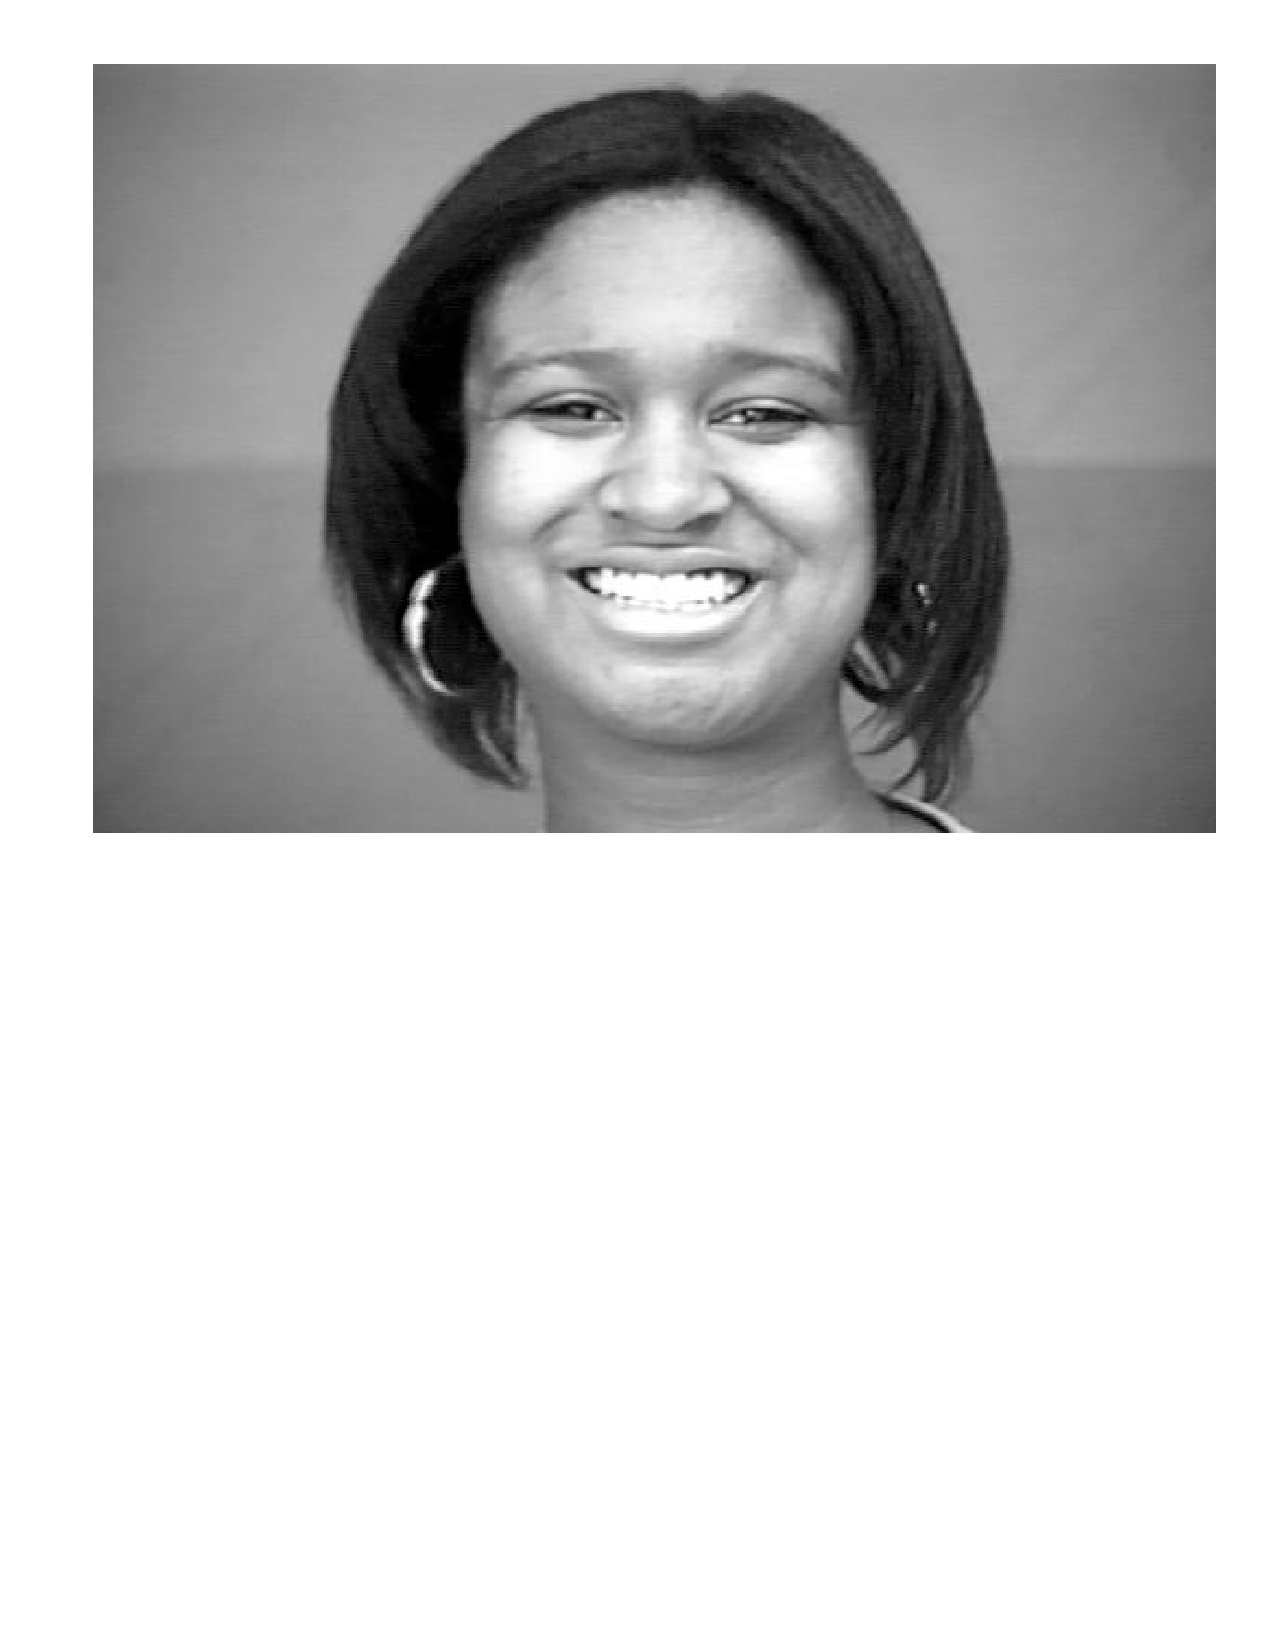
\includegraphics[width=\textwidth]{ME32}
      \caption{}
    \end{subfigure}
    \begin{subfigure}[b]{0.22\textwidth}
      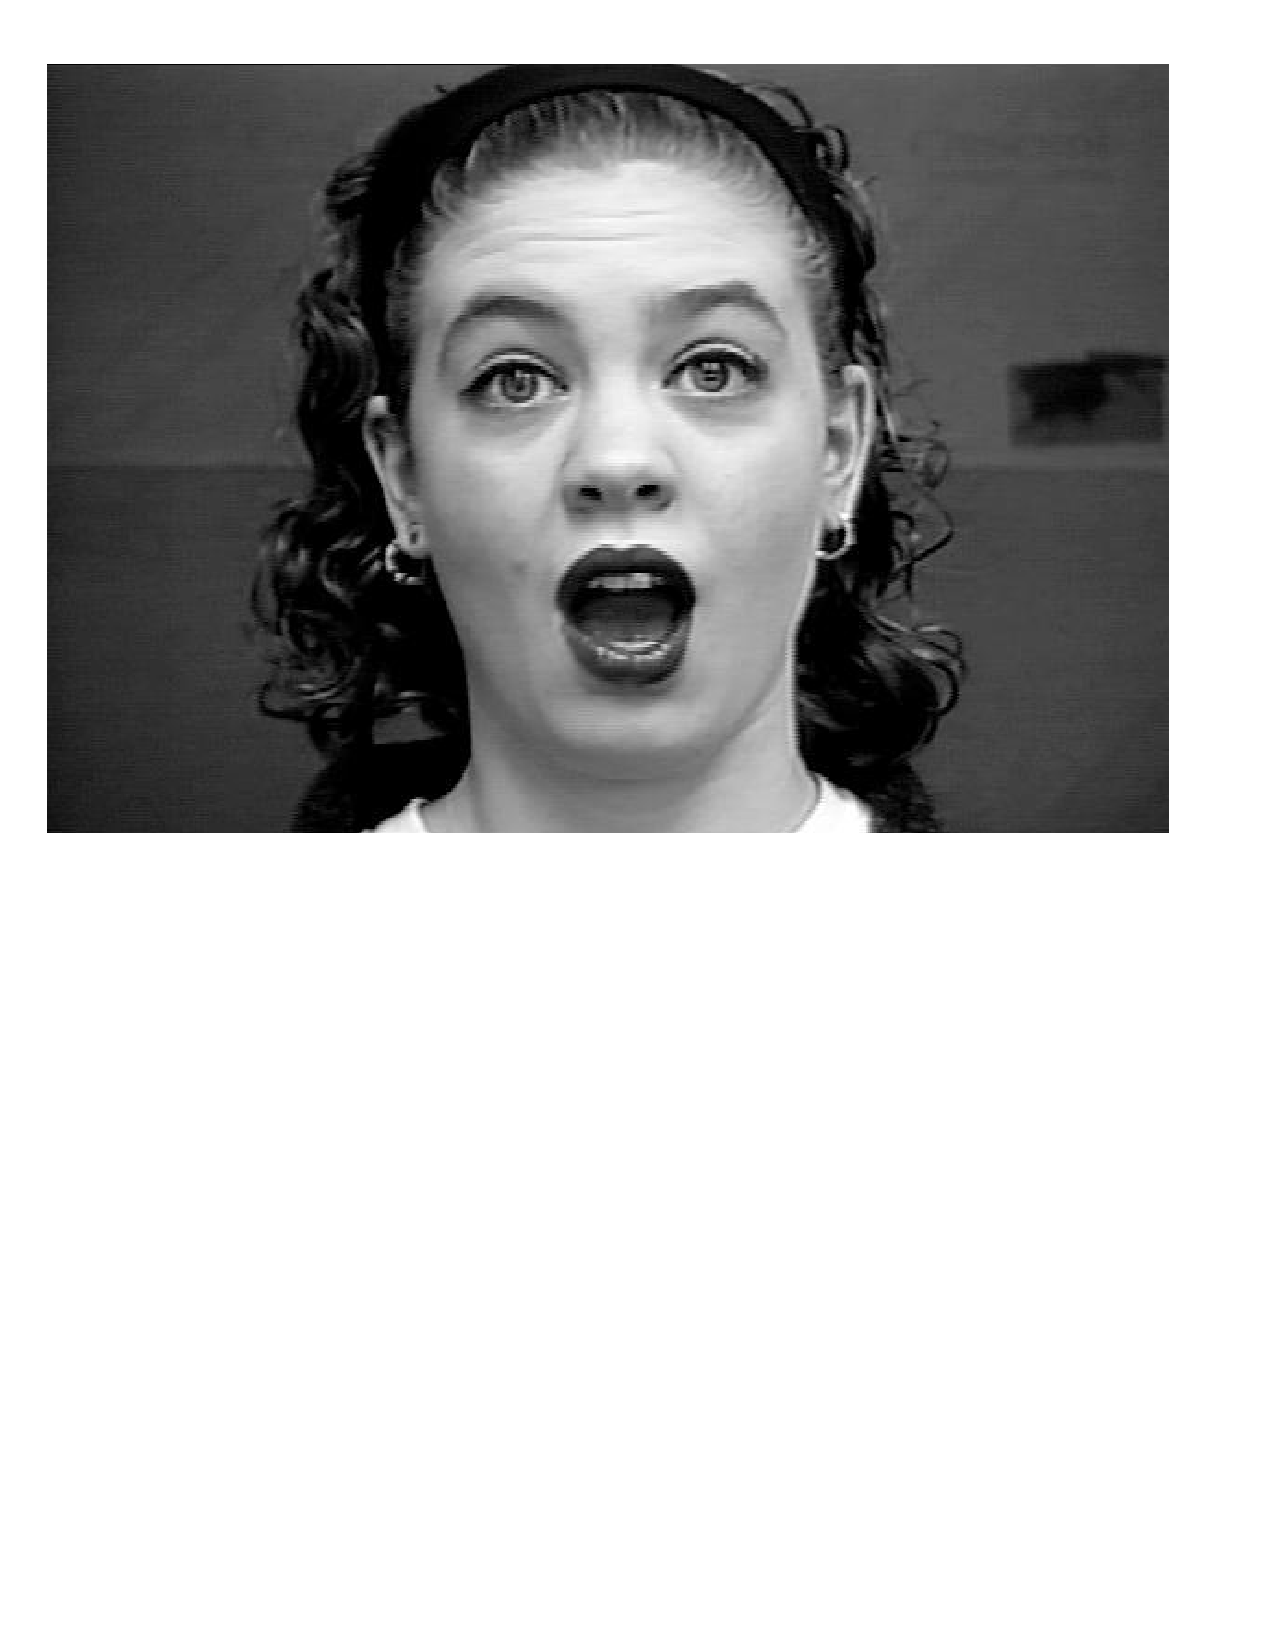
\includegraphics[width=\textwidth]{ME33}
      \caption{}
    \end{subfigure}%
    ~%add desired spacing
    \begin{subfigure}[b]{0.22\textwidth}
      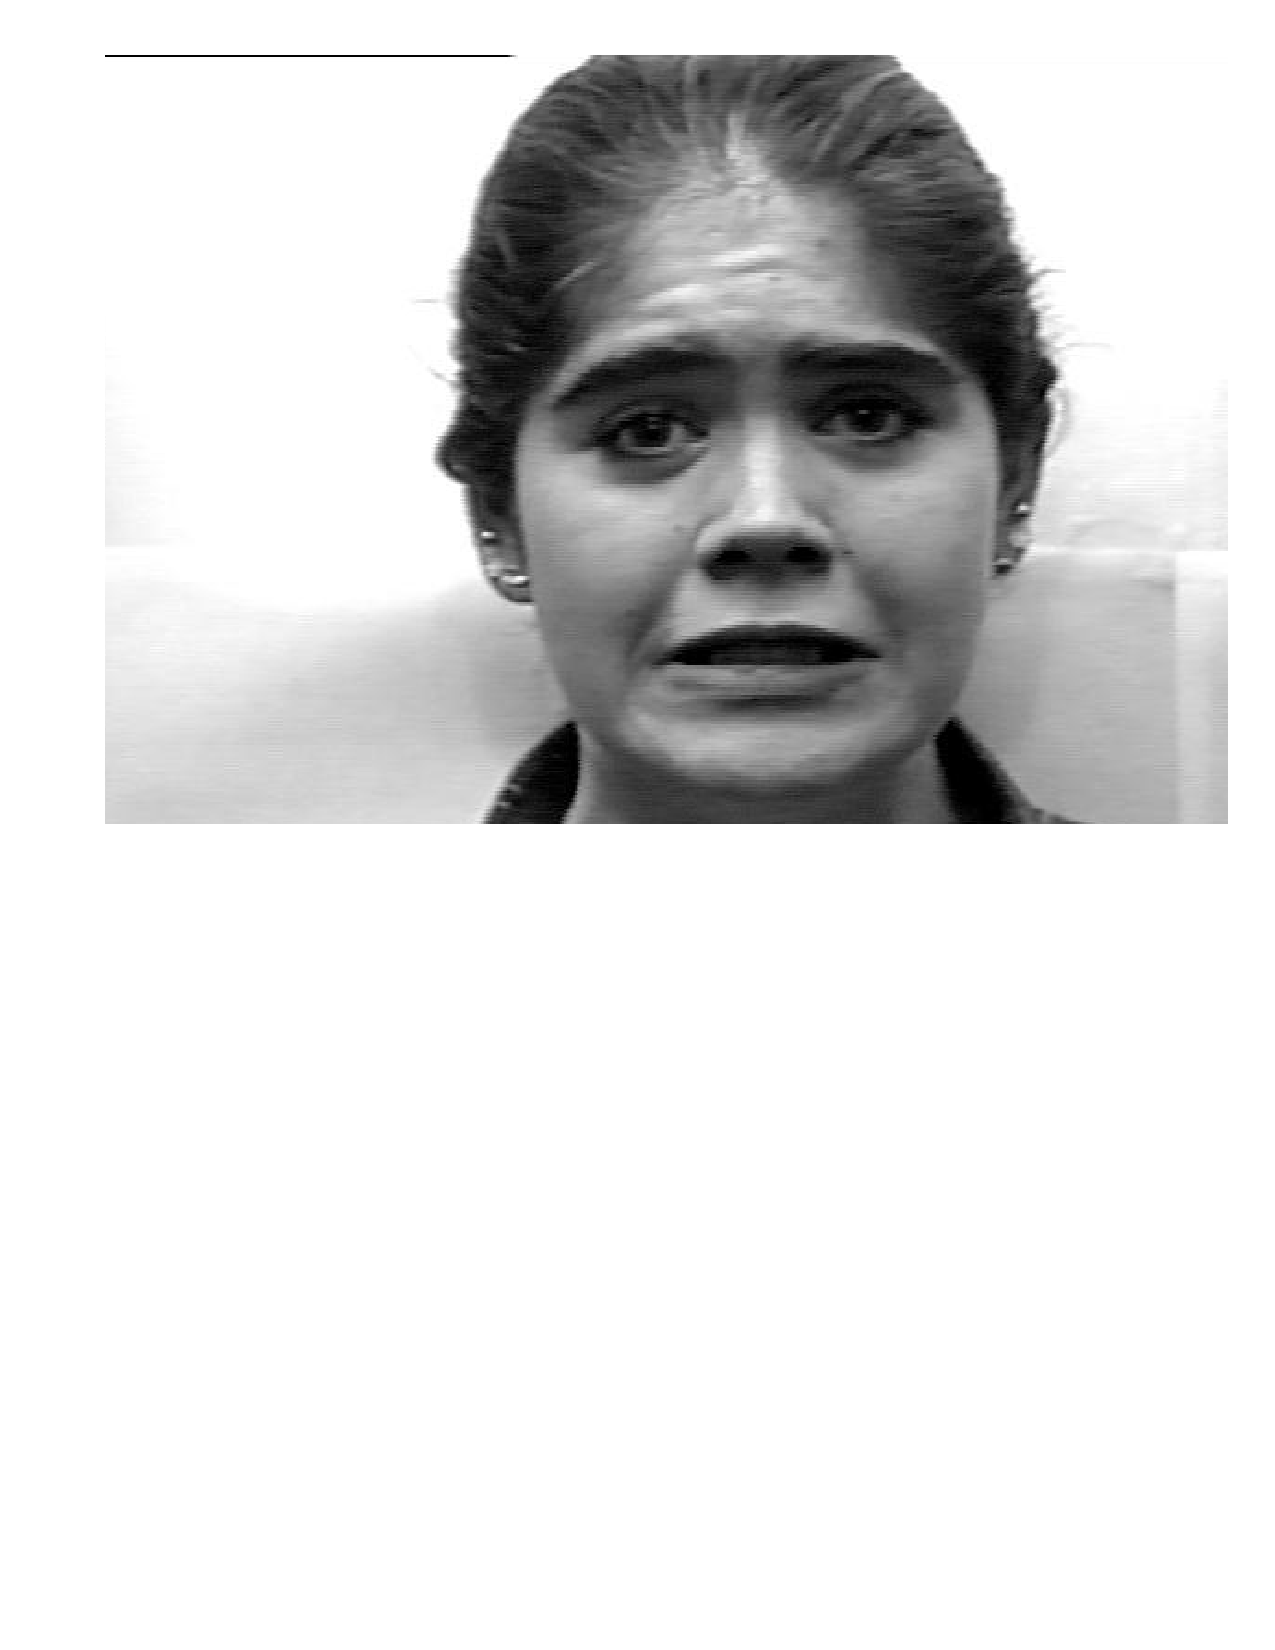
\includegraphics[width=\textwidth]{ME34}
      \caption{}
    \end{subfigure}
    \begin{subfigure}[b]{0.22\textwidth}
      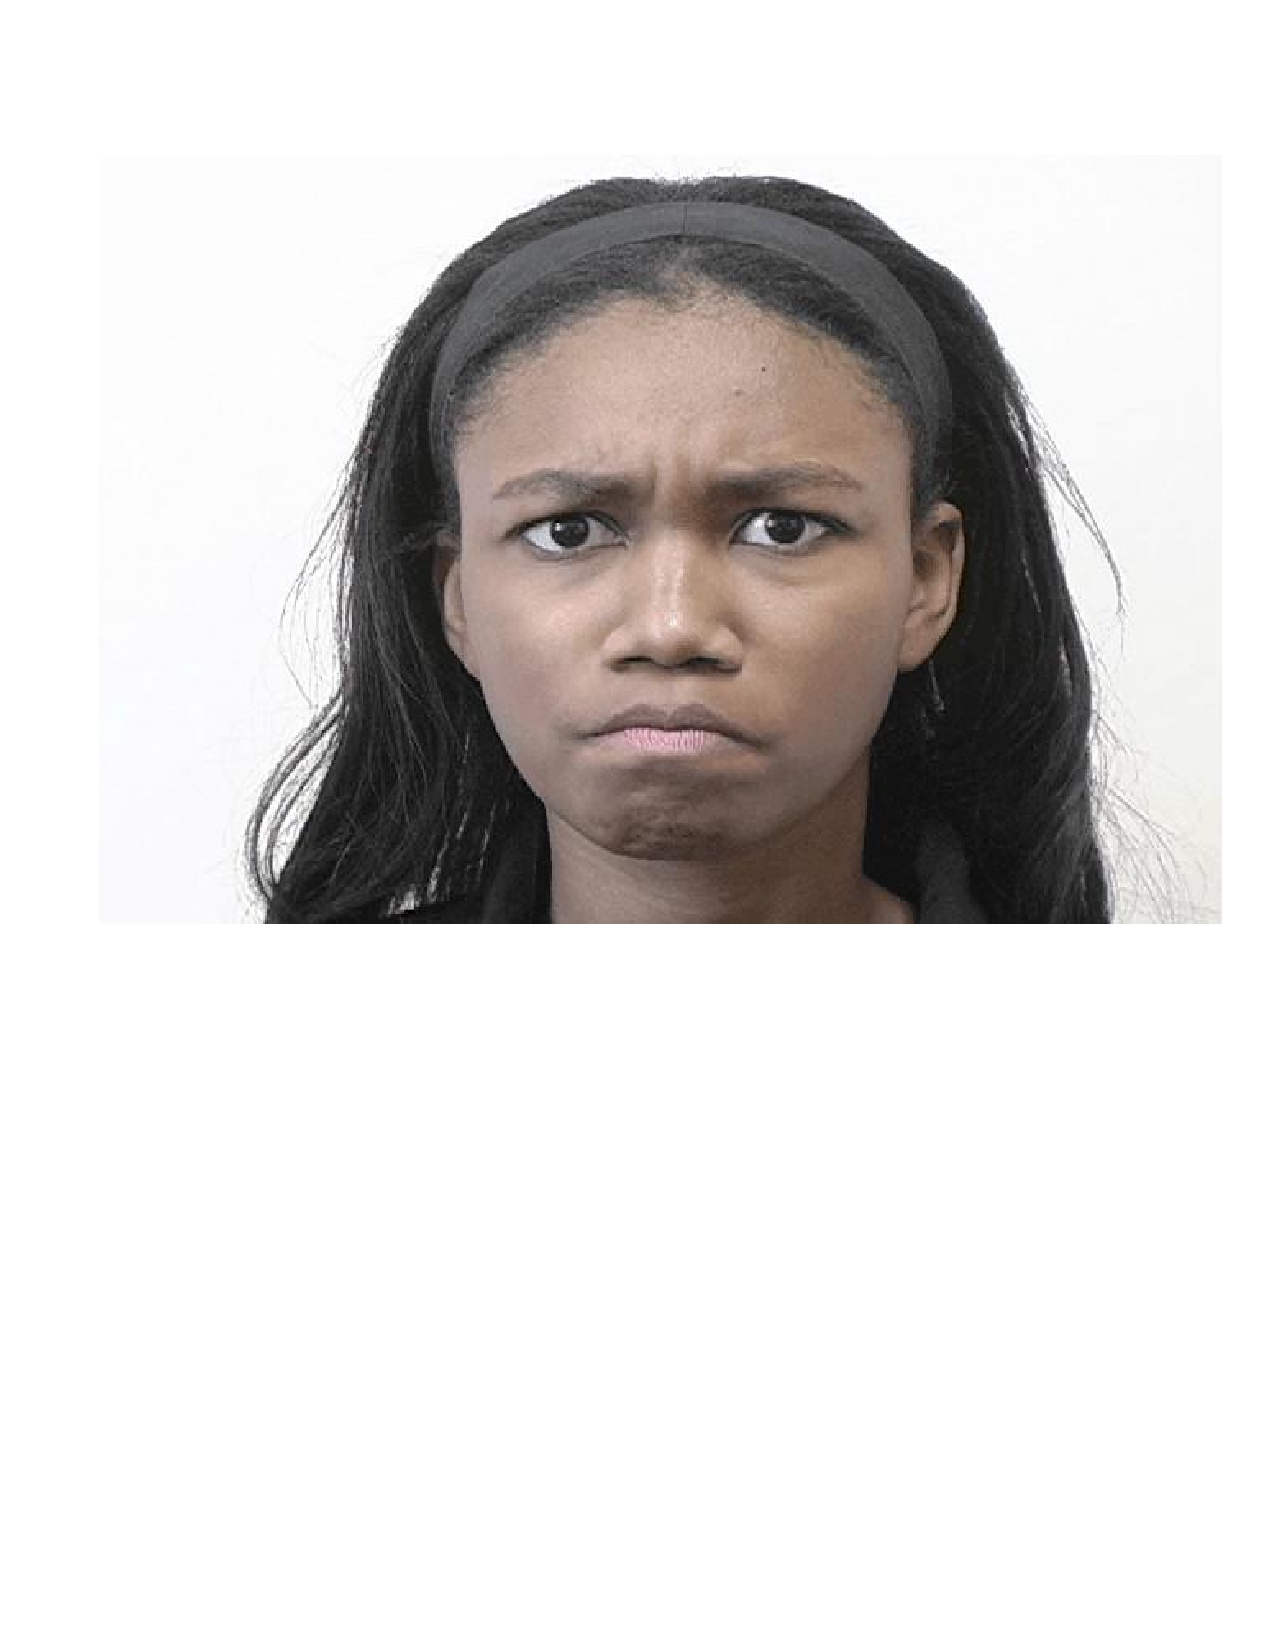
\includegraphics[width=\textwidth]{ME35}
      \caption{}
    \end{subfigure}
    \begin{subfigure}[b]{0.22\textwidth}
      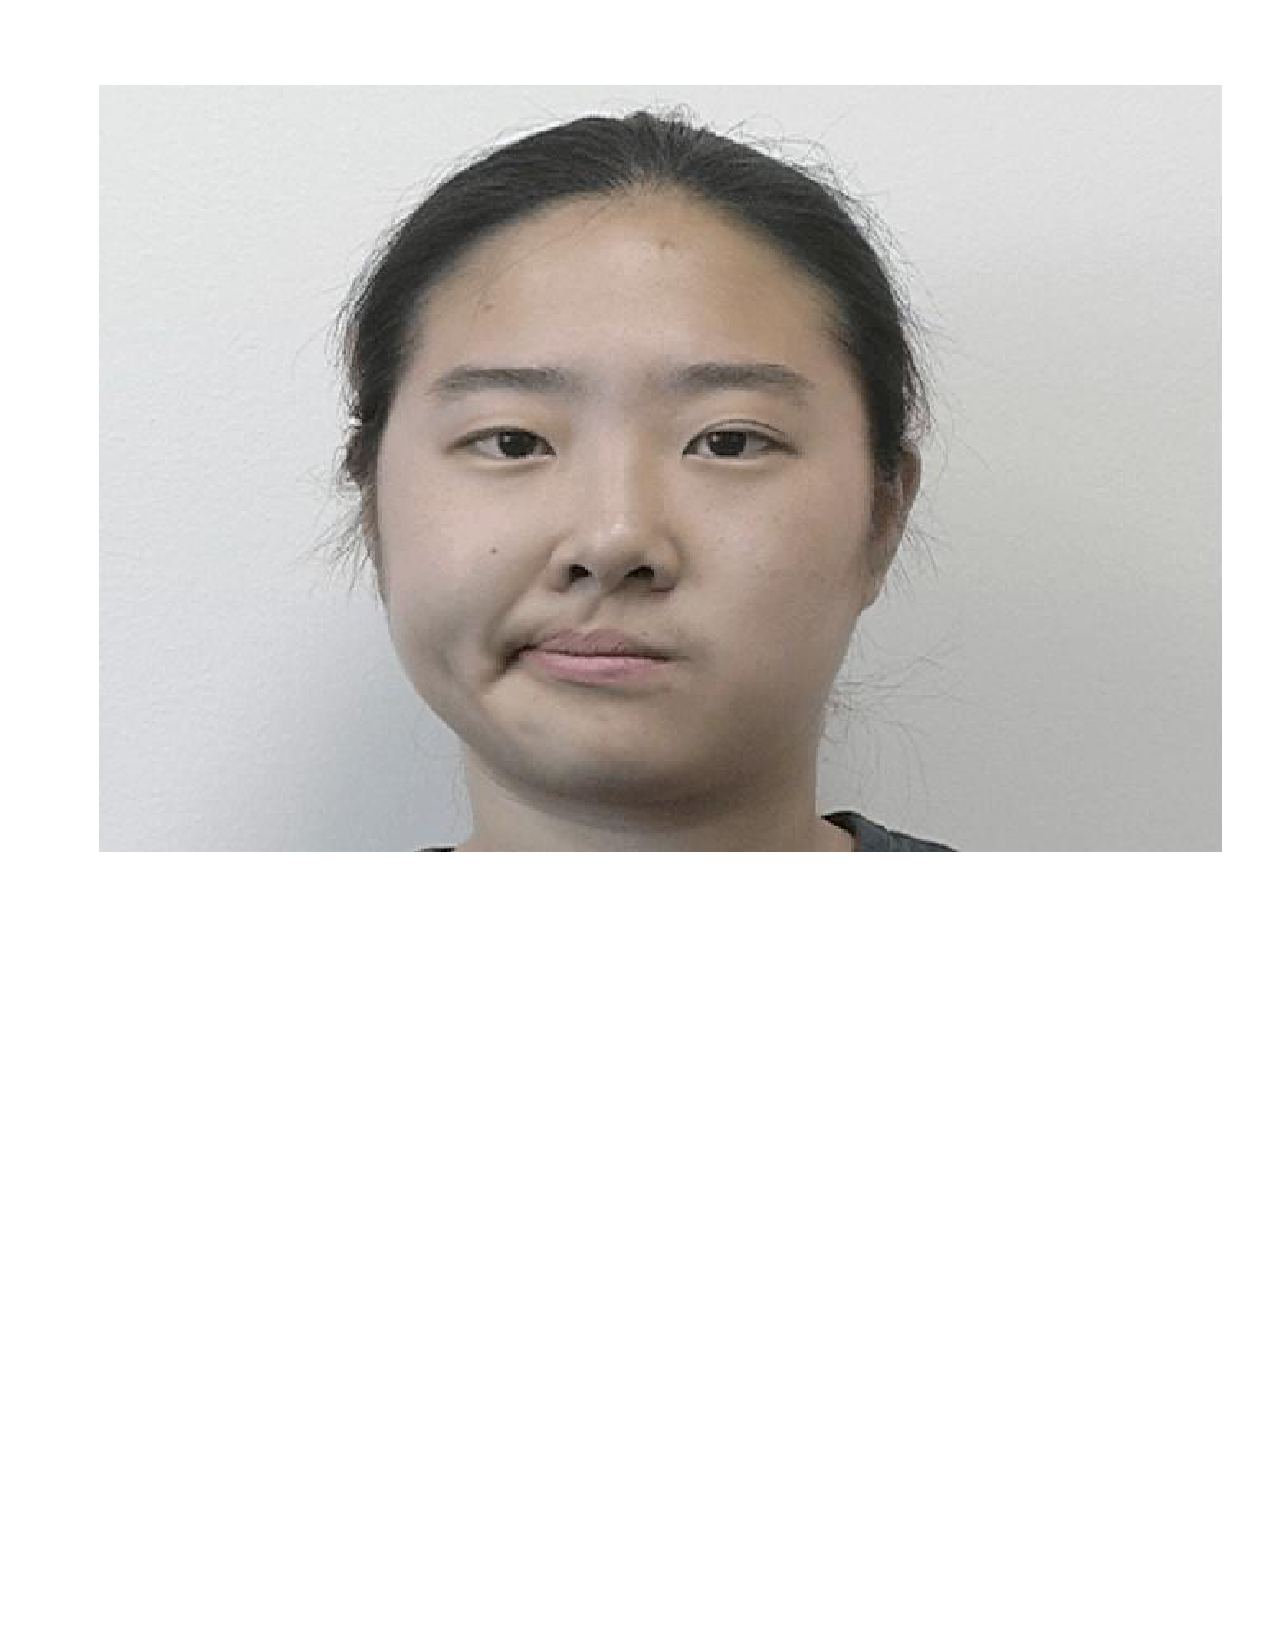
\includegraphics[width=\textwidth]{ME36}
      \caption{}
    \end{subfigure}
    \begin{subfigure}[b]{0.22\textwidth}
      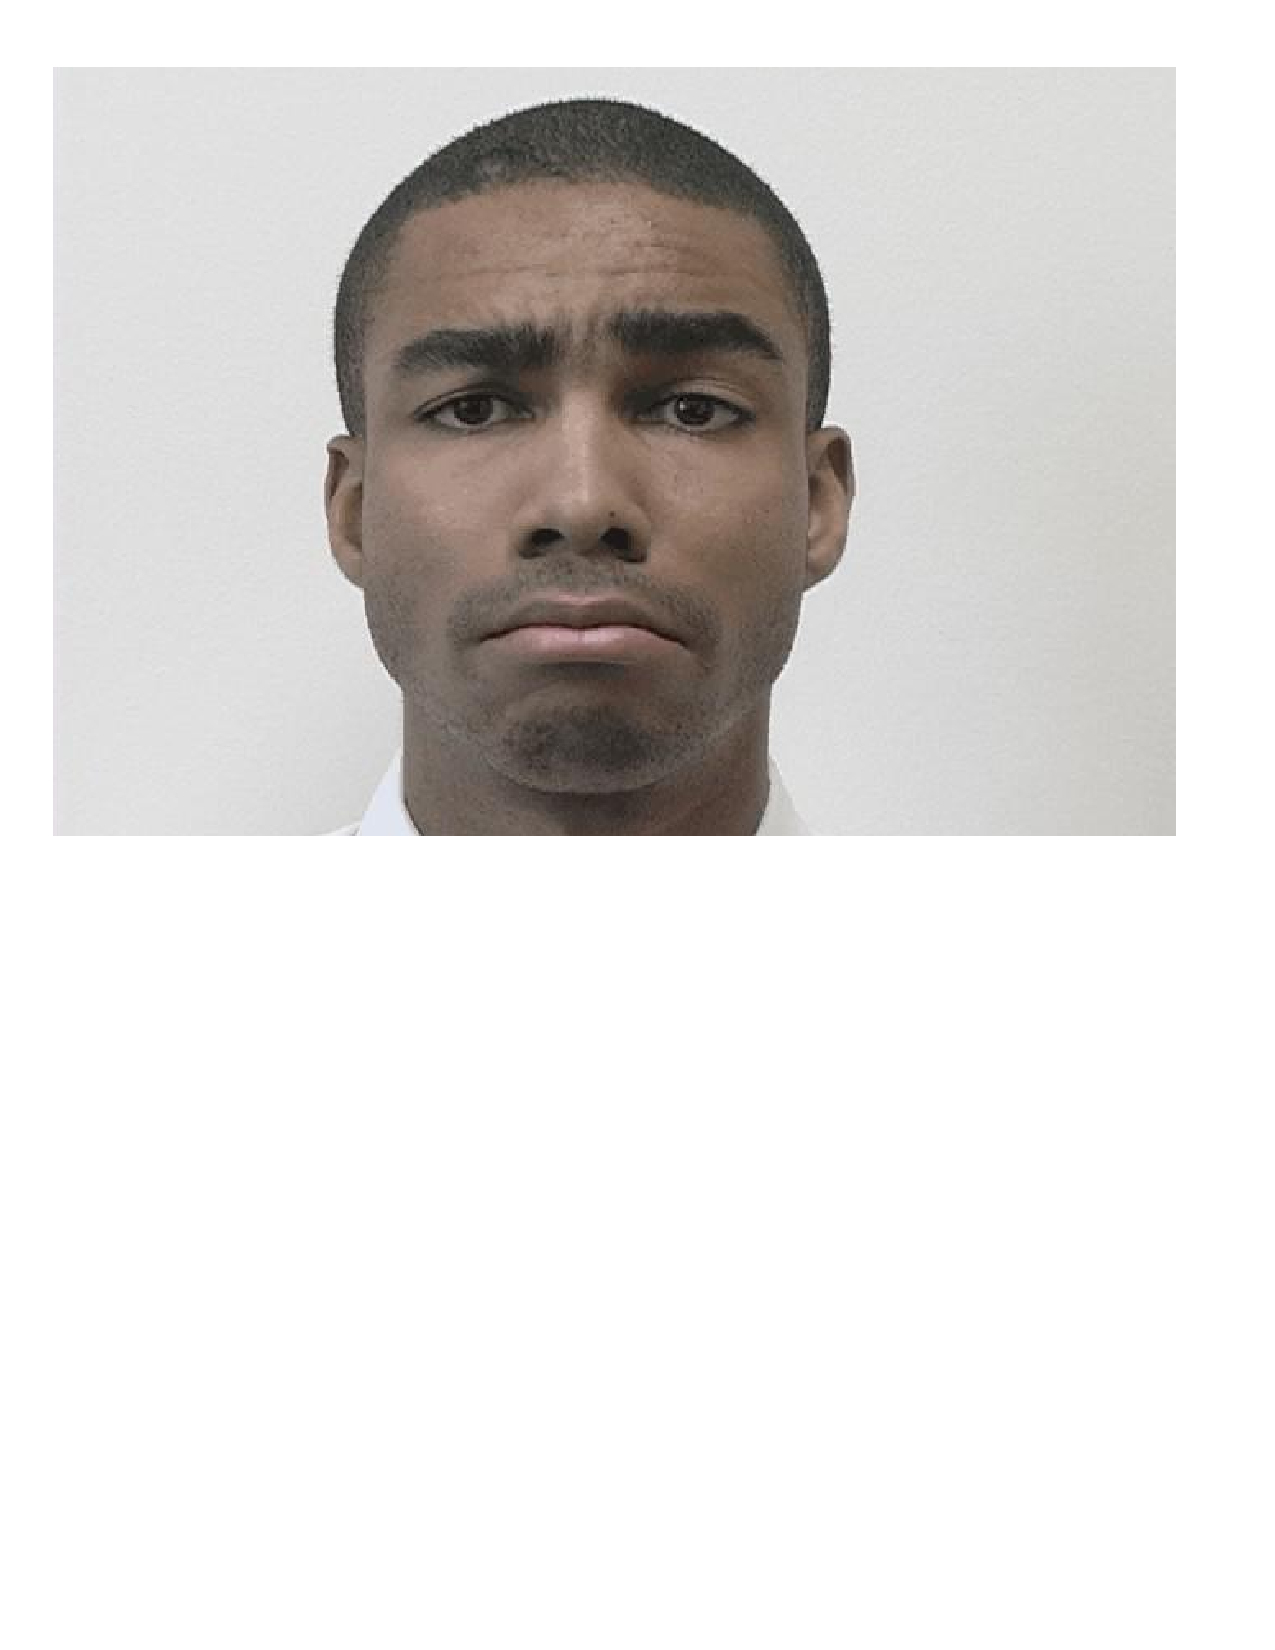
\includegraphics[width=\textwidth]{ME37}
      \caption{}
    \end{subfigure}
    \begin{subfigure}[b]{0.22\textwidth}
      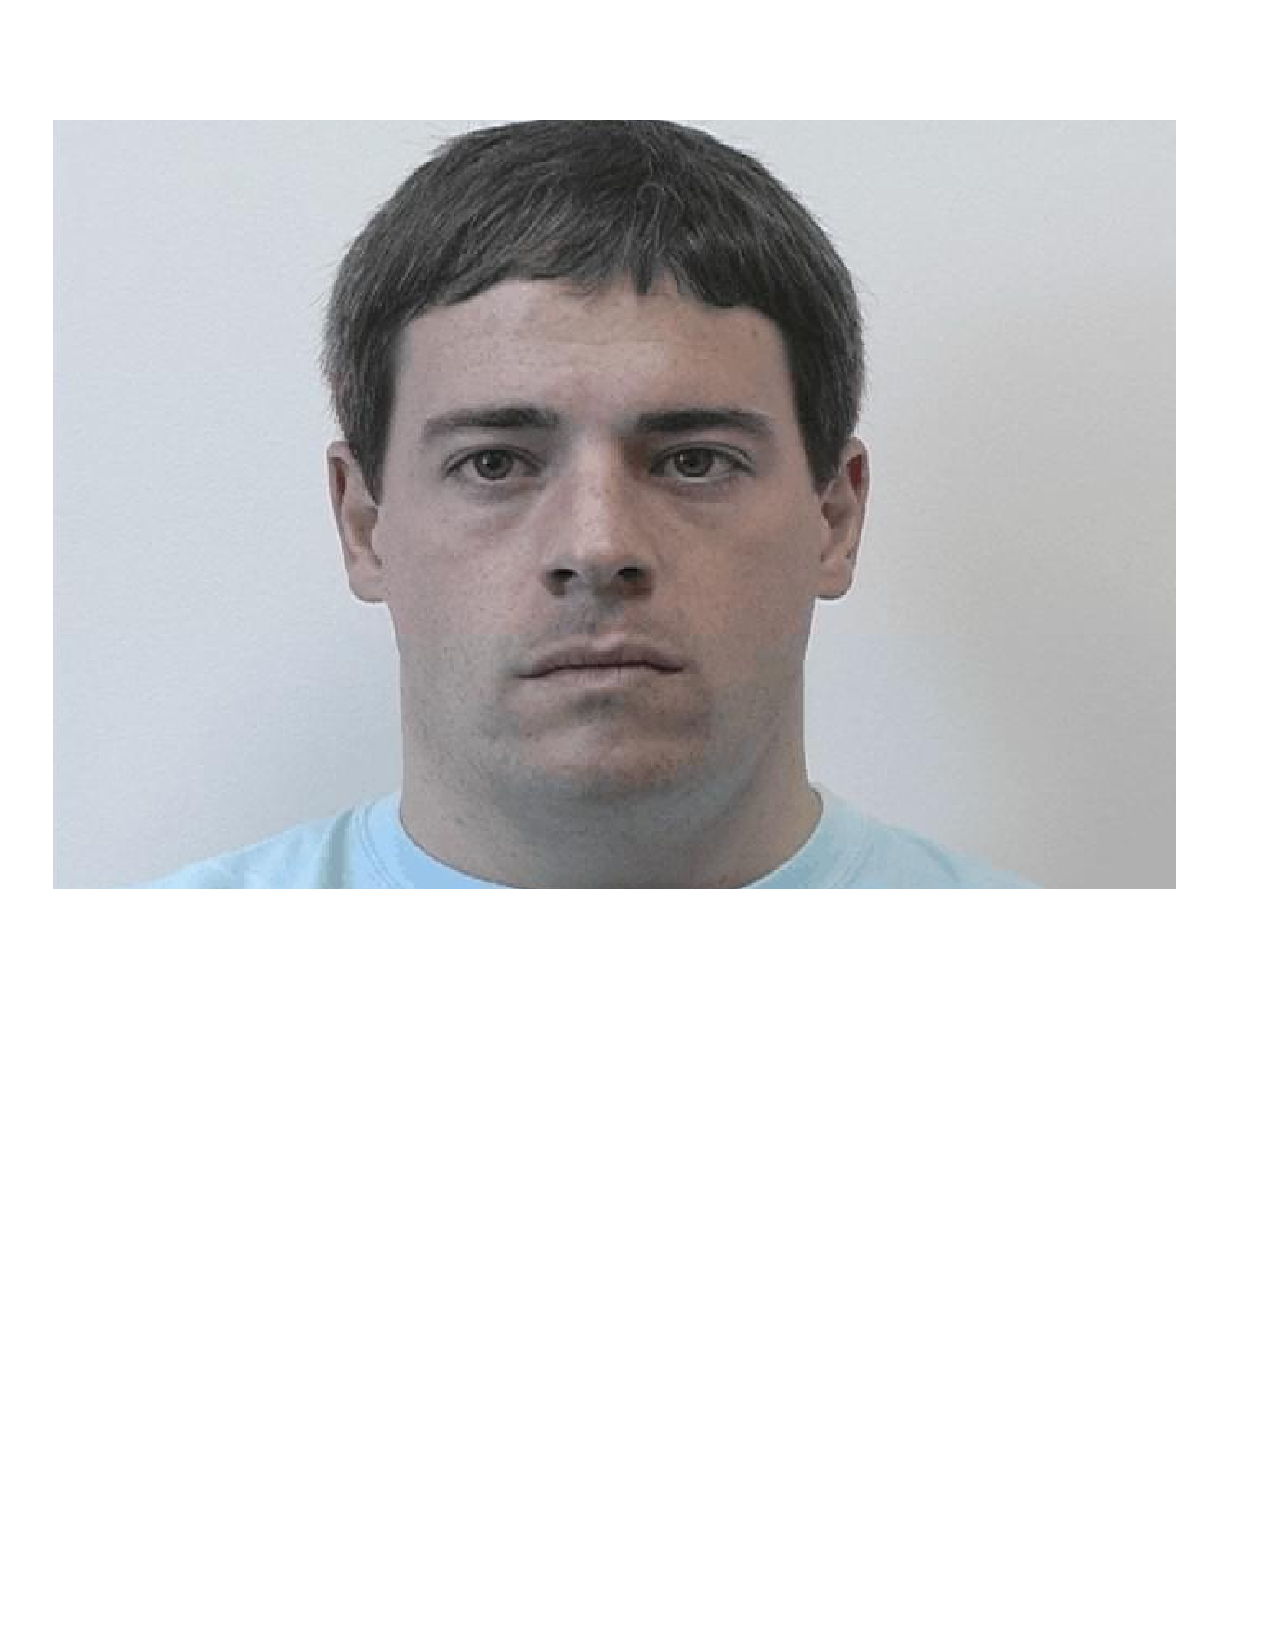
\includegraphics[width=\textwidth]{ME38}
      \caption{}
    \end{subfigure}
    \begin{spacing}{1.0}
    \caption{人脸宏表情样本示例(CK+数据集)}
    \label{fig1}
    \centerline{\footnotesize \textmd{(a)厌恶、(b)快乐、(c)惊讶、(d)压抑、(e)生气、(f)蔑视、(g)厌恶、(h)中性表情}}
    \end{spacing}
\end{figure}

\subsection{早期微表情数据集}

由于微表情在镜头下很难产生,所以微表情数据的缺乏是微表情研究的第一障碍。虽然微表情已经被心理学家研究了很长一段时间,但网络上广泛传播的微表情样本仅仅只有片段,并没有发现任何心理学研究小组分享的大数据集。作者认为第一个原因是心理学研究更关注微表情本身的性质,比如什么时候出现或者看起来是什么样子,所以他们不需要像使用计算机研究那样需要大量的微表情数据。其次,在某些情况即使涉及到大量的微表情数据,但由于保密性限制,数据无法公开共享,例如患者的病历或司法讯问记录等。

以2009年为时间点,在此以前属于微表情的早期研究阶段,一些研究人员在他们的研究中使用了摆拍的微表情数据,这些数据避免了自发微表情数据获取时的困难,作为早期自动微表情识别研究的尝试,使用摆拍的数据是一次历史性的突破。例如Shreve等人收集了一个名为USF-HD的数据集,其中包含100个摆拍的微表情片段,视频长度平均在1分钟左右,最长2分钟,最短20秒。研究人员要求参与者模仿屏幕上显示的微表情样本作为数据的来源,同时在他们的文章中明确写到可以通过要求参与者尽可能快地模仿来收集一个摆拍的微表情数据集。Polikovsky等人也收集了一个摆拍的微表情数据集,要求受试者在低强度下表演七种基本情绪,并尽快回到中性表情,数据由一台每秒200帧的高速摄像机记录。表~\ref{tab2}列出了摆拍的微表情数据集的详细属性。

\begin{table}[!htbp]
\renewcommand\arraystretch{1.5}
\centering
\caption{摆拍微表情数据集}
\label{tab2}
\footnotesize% fontsize
\setlength{\tabcolsep}{5pt}% column separation
\begin{tabular}{c|cc}
\hline
 & USF-HD & Polikovsky \\ \hline
微表情片段 & 100 & N/A \\
参与者 & N/A & 10 \\
分辨率 & $720\times1280$ & $480\times640$ \\
FPS & 29.7 & 200 \\
FACS & NO & YES \\
表情类 & N/A & 7 \\
人种 & N/A & 3 \\ \hline
\end{tabular}
\end{table}

值得注意的是摆拍的微表情数据不可以代替或与自发的微表情数据一起使用,因为这两种数据是不同性质的。例如在研究微表情的起始点时,由于两者是在不同的机制下产生的,所以摆拍的微表情在时空特性上与自发的微表情存在很大的差异,其次在研究视频的上下文时,由于模仿的表情与通过视频编辑生成的摆拍微表情片段通常在起止点很突兀,而且期间禁止其他无关的动作发生,这也与自发的微表情有很大的不同。另一方面,自然环境下自发的微表情可能伴随着复杂的场景,比如头部运动和眨眼等动作。基于这些事实,利用摆拍的微表情数据进行研究并不能真正解决实际中微表情分析的自动化问题,所以努力收集自发的微表情数据是后续工作的正确路径。需要说明的是在本文接下来的内容中,所有的工作都是关于自发微表情的,如果没有特别说明,“微表情”一词表示自发微表情。

\subsection{自发微表情数据集}

A. SMIC数据集介绍

2011年,论文\citepns{pfister2011recognising}首次提出了一种诱导和收集自发微表情的方法,将获得的数据集命名为“自发微表情语料库”,简称SMIC,它是第一个使用
自然诱发状态的微表情数据集,对后续的数据集建立具有很好的指导性意义。第一版的SMIC数据集只包含了6位参与者的数据,论文\citepns{Li2013A}对其进行了扩充,包含
了16名参与者的164个自发微表情片段,由三种相机记录的3个数据集组成:100fps的高速相机记录的HS数据集、25fps的普通彩色相机记录的VIS数据集和25fps的近红外摄像机记录的NIR数据集,且所有数据集具有相同的图像分辨率$640\times480$。增加VIS和NIR摄影机有三个考虑:(1)提升数据集的多样性;(2)研究高速相机在微表情分析方面是否优于普通速度相机;(3)研究时间插值方法是否可以应用于普通高速相机,以解决相机的短时插值问题。图~\ref{fig2}给出一个消极的微表情序列,通过该样例可以看出,一个微表情是由一组图片序列构成的,本样例的变化主要表现为嘴角的细微下沉。

\begin{figure}[!htbp]
    \centering
    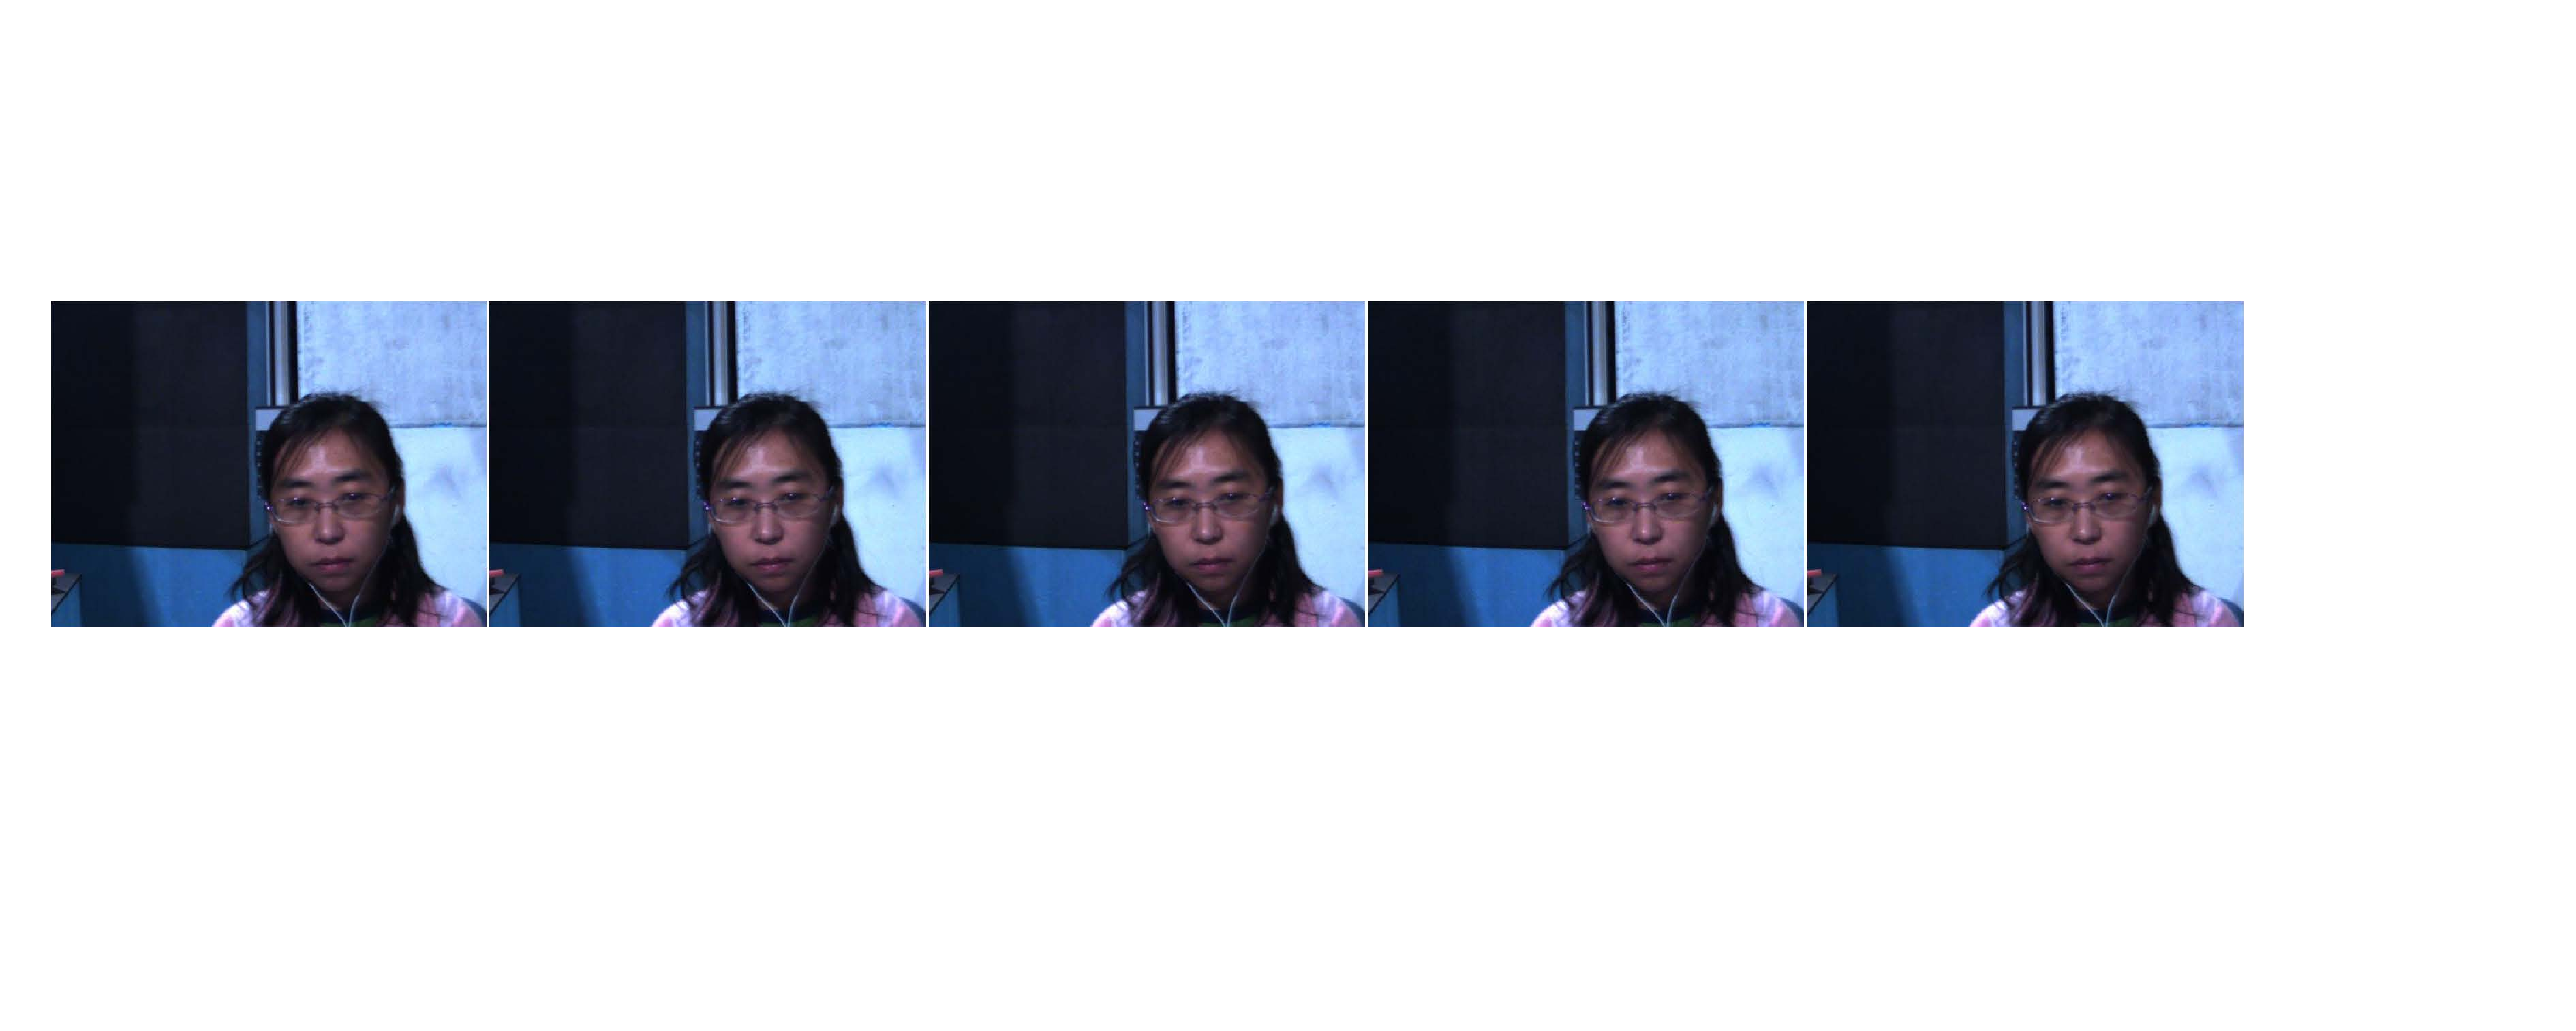
\includegraphics[width=0.95\textwidth]{ME1}
    \caption{一个消极的微表情片段示例(SMIC数据集)}
    \label{fig2}
\end{figure}

a)视频采集

研究表明通过图像、视频和音乐等一定的刺激能够诱发真实的表情\citep{Coan2015Handbook}。自发微表情是由人的内心感受触发的非自愿行为,所以可以使用上述方法引发情感反应。但必须找到一种能确保诱发的表情足够短的方法(满足微表情的标准)。一些心理学著作研究了微表情发生的条件,Ekman等人认为当人们试图隐藏自己的真实情感时,尤其是当被抓住后果会很严重时,微表情就会出现,这被称为高风险条件,例如嫌疑人正在接受警察或测谎专家的审问,这是一种很自然的高风险场景。但是对于采集数据而言,营造真正的审问现场显的不太可能。所以为了诱导参与者自发的微表情,需要找到一种模拟高风险环境的方法。设计的情景必须满足以下两个要求:(1)激发参与者情绪的刺激必须有效,使激发的情绪反应强烈到无法完全隐藏;(2)应该制造高压力,这样参与者才会有动力去尽力隐藏自己的真实感受。

作者使用了心理学研究中诱导抑制情绪产生的方法。采集前向参与者详细说明研究内容和过程,显示器上显示如下提示性语句:“(1)将向您展示几段诱发情绪的短片,请尽量保持头部稳定并仔细观看。(2)每段视频片段后,您将有一个短暂的休息。请根据您对刚才看到的视频的真实感受填写调查表(报告中的情感反馈是标注过程中的重要参考。)。(3)当您在看视频的时候,我会待在另一个房间,通过摄像头观察您的面部和身体动作,并尝试猜测您所看的视频片段(片段是随机播放的)。您的任务是装出若无其事的样子,而不是表露您的真实感情。如果您不能隐藏您的感觉,您将不得不填写一份超过500个冗长而乏味的问题问卷。”

在每段影片结束后,参与者将在问卷中回答以下问题:“(1)您在看视频时感受到了什么样的情绪(快乐、悲伤、厌恶、压抑、惊讶、愤怒或困惑)?(2)看视频的时候您是否感觉到愉悦?(从1到7愉悦程度逐渐上升)”。选择最有效的刺激作为情感诱导因子是后续数据采集的关键因素之一。通过查阅文献比较不同类型的情绪诱导材料,如图像、音乐、视频和互动。最终决定使用短视频作为微表情采集诱导剂的原因有三个:(1)视频包含音频和视觉信息,因此比图像和音乐的影响更强大;(2)视频能够持续一段时间,更能激发强烈情绪,更容易产生微表情;(3)从获取稳定额叶面部视频的实际角度来看,观看视频的参与者比多人参与的互动场景更容易控制。

20名来自奥卢大学的学生和研究人员自愿参与数据集的制作,参与者的年龄从22岁到34岁不等,其中7位是女性,13位是男性,9人是白种人,11人是亚洲人。研究人员在电脑显示器上向参与者展示了16段精心挑选的能引发强烈情绪的视频片段。当参与者观看视频片段时,三个固定在电脑显示器上的摄像头记录参与者的面部反应,操作人员在前方通过另外一台电脑监控参与者的面部反应,图~\ref{fig3}给出了环境设置示意图。

\begin{figure}[!htbp]
    \centering
    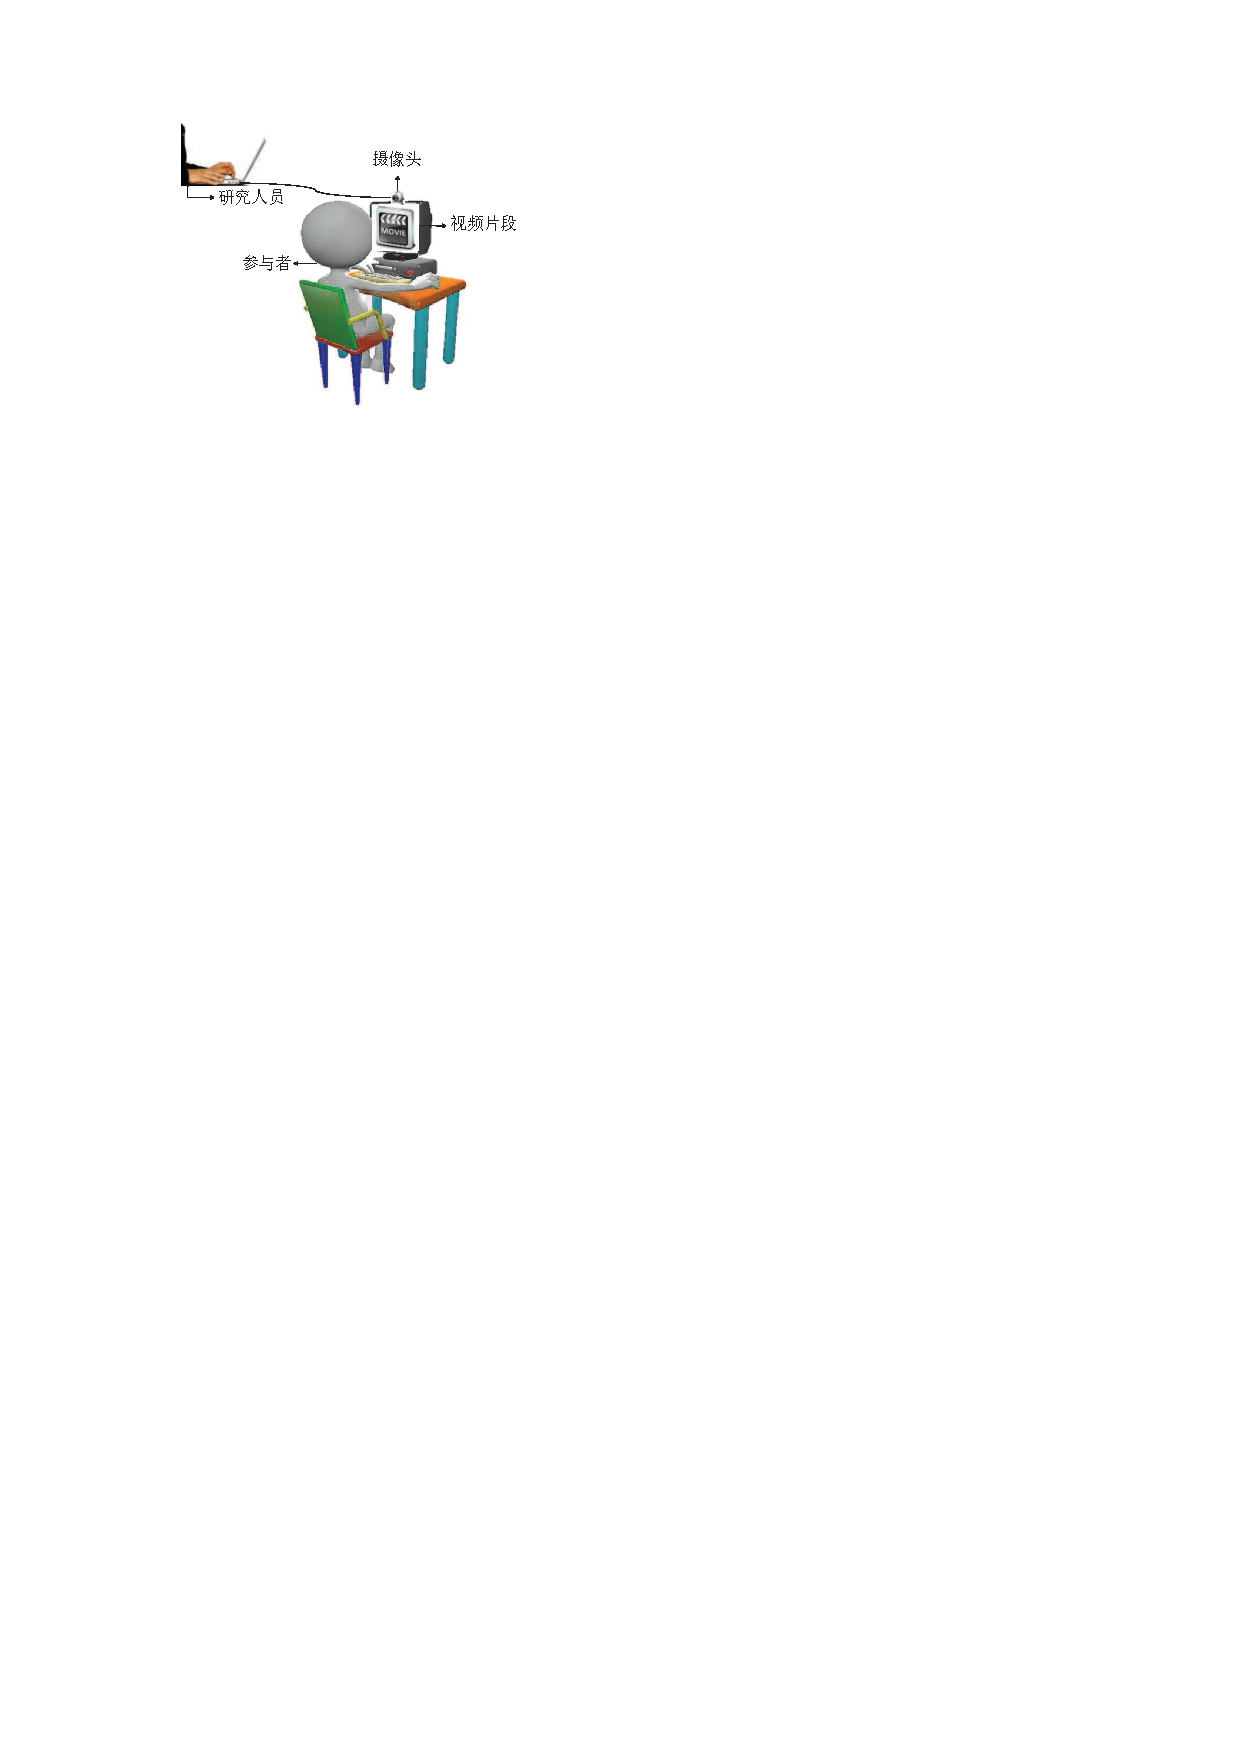
\includegraphics[width=0.45\textwidth]{collect}
    \caption{微表情数据采集示意图}
    \label{fig3}
\end{figure}

b) 视频的标注

录制的视频需要进行分割和标注,目的是得到适合研究人员进行训练与测试的微表情样本和相应的标签。采集的三种视频中高速视频由于具有最佳的时间分辨率所以非常适合标注,另外两个摄像头拍摄的视频需要同步后再进行标注。首先,从原始的长视频中分割出微表情的起始和终止帧,微表情序列的开始表示的是与之前中立(或接近中立)的人脸表情相比的可见运动的第一帧,而微表情序列的终止指在与下一帧相比可以发现任何运动时结束的最后一帧。关于微表情精确的长度限制目前还存在争议,SMIC数据集参考论文\citepns{Yan2013How}和 \citepns{matsumoto2011evidence}等人的建议,设置了1/2秒较宽松的分割节点。注意,并不是所有的微表情都结束于一个完全的中性表情,有些表情可能会上升,然后下降到接近中性的状态,并保持这种状态很长时间,这也被认为是微表情的结束。

随后,对所有的视频片段都用情感标签进行标注。情感标签的证据有两种:视频片段的内容和参与者提交的报告。虽然在视频播放前已经预知将可能产生某种确定情绪,但研究发现,参与者在某些视频刺激下可能会产生不同的情绪表现(甚至相反的情绪)。在少数情况下,当参与者提交的问卷报告与视频内容相反时(例如,一些参与者反馈在观看恐怖视频片段时感到快乐或有趣),SMIC数据集使用参与者的提交的报告作为微表情标签的标准。起初,SMIC数据集根据视频内容分配了五种情感标签,包括快乐(Happy)、悲伤(Sad)、恐惧(Fear)、厌恶(Disgust)和惊讶(Surprise)。后来,SMIC数据集将五类标签合并为三类:积极(Positive)、惊讶(Surprise)和消极(Negative)。将第一版本的快乐类别改为新的积极类别,而消极类别则是由第一版的悲伤、恐惧和厌恶这三个类别组合而成。将三种消极情绪融合在一起的原因是:首先,参与者在该段视频的报告中选择了三种情绪中的一种以上;其次,三种标签的样本量都太小,合并后会更好的平衡。根据具体情况,惊讶类别可以分为积极惊讶和消极惊讶。同时为了验证数据标签的有效性,标注由两位标注者分别执行。然后,两位标注者相互交换检查各自的标注,只有当两位标注者的标注结果一致时的标签有效。

B. CASME数据集介绍

在SMIC发表后不久,另一组研究人员收集了新的自发微表情数据集。由中国科学院Yan等人采用与SMIC相似的情绪诱导方式收集了中国科学院微表情数据集(CASME),包含19位中国籍参与者的195个微表情片段。CASME由两台相机记录,一台是明基M31相机,帧率为60fps,分辨率为$1280\times720$(CASME-A),另一台是灰点GRAS-03K2C相机,帧率为60fps,分辨率为$640\times480$(CASME-B)。CASME数据集中的微表情首先使用AU标记,然后被分为八类情绪,包括娱乐(Amusement)、悲伤(Sadness)、厌恶(Disgust)、惊讶(Surprise)、蔑视(Contempt)、压抑(Repression)、恐惧(Fear)和紧张(Tension)。之后又发布了第二版数据集CASME II,CASME II提供了更多具有更高时空分辨率的微表情样本。新数据集的平均人脸尺寸为$280\times340$,每秒200帧,是从26名中国参与者中获得的247个微表情样本。CASMEII样本有五个类的AU标签和情感标签,即开心(Happiness)、厌恶(Disgust)、惊讶(Surprise)、压抑(Repression)和其他(Others)。

CASME II数据集相比之前的数据集引入了AU标签,它是在充分考虑了主客观因素(除了FACS编码的基本判断)外,还参考了参与者自己的主观回忆来辅助标注的样本标签。除此之外,该数据集还对微表情的起始帧、峰值帧和终止帧都做了详细的标注。

C. 其他数据集介绍

最近又有一个新的自发微表情数据集SAMM发布,它也使用了类似于SMIC和CASME的情绪诱导方法,从13个不同民族的32名参与者中获得159个微表情。SAMM数据具有更高的帧分辨率$2040\times340$,帧速率为200fps。数据提供了AU标签和八种表情标签,包括开心(Happiness)、惊讶(Surprise)、悲伤(Sadness)、生气(Anger)、恐惧(Fear)、厌恶(Disgust)、蔑视(Contempt)和其他(Other)。

表~\ref{tab3}列出了当前所有提到的微表情数据集的详细参数。

\begin{table}[!htbp]
  \renewcommand\arraystretch{1.5}
  \centering
  \caption{自发微表情数据集}
  \label{tab3}
  \footnotesize% fontsize
  \setlength{\tabcolsep}{4pt}% column separation
    \begin{tabular}{c|cccccc}
    \hline
     & SMIC-HS & SMIC-subHS & SMIC-NIR & SMIC-VIS & CASME II & SAMM \\ \hline
    微表情片段 & 164 & 71 & 71 & 71 & 247 & 159 \\
    参与者 & 16 & 8 & 8 & 8 & 26 & 32 \\
    分辨率 & $640\times480$ & $640\times480$ & $640\times480$ & $640\times480$ & $640\times480$ & $2040\times1088$ \\
    人脸分辨率 & $190\times230$ & $190\times230$ & $190\times230$ & $190\times230$ & $280\times340$ & $400\times400$ \\
    FPS & 100 & 100 & 100 & 100 & 200 & 200 \\
    性别比(F/M) & 6/10 & 2/6 & 2/6 & 2/6 & 15/11 & 16/16 \\
    FACS & NO & NO & NO & NO & YES & YES \\
    表情类 & 3 & 3 & 3 & 3 & 5 & 8 \\
    平均年龄(SD) & 26.7(N/A) & 26.7(N/A) & 26.7(N/A) & 26.7(N/A) & 22.03(SD=1.6) & 33.24(SD=11.32) \\
    人种 & 2 & 2 & 2 & 2 & 1 & 4 \\ \hline
    \end{tabular}
\end{table}

\subsection{宏表情与微表情比较}

通过前两小节的介绍可以看出微表情和宏表情最大的区别是在面部肌肉的运动强度和持续时间。如图~\ref{fig4}所示,人脸根据不同的部位被划分为不同的肌肉组如皱眉肌、
降眉间肌、鼻肌等,图~\ref{fig1}中上述肌肉运动明显比图~\ref{fig2}更加剧烈也更加夸张;另一方面,微表情的持续时间一般在1/25秒到1/2秒之间,而宏表情则不然。

\begin{figure}[!htbp]
    \centering
    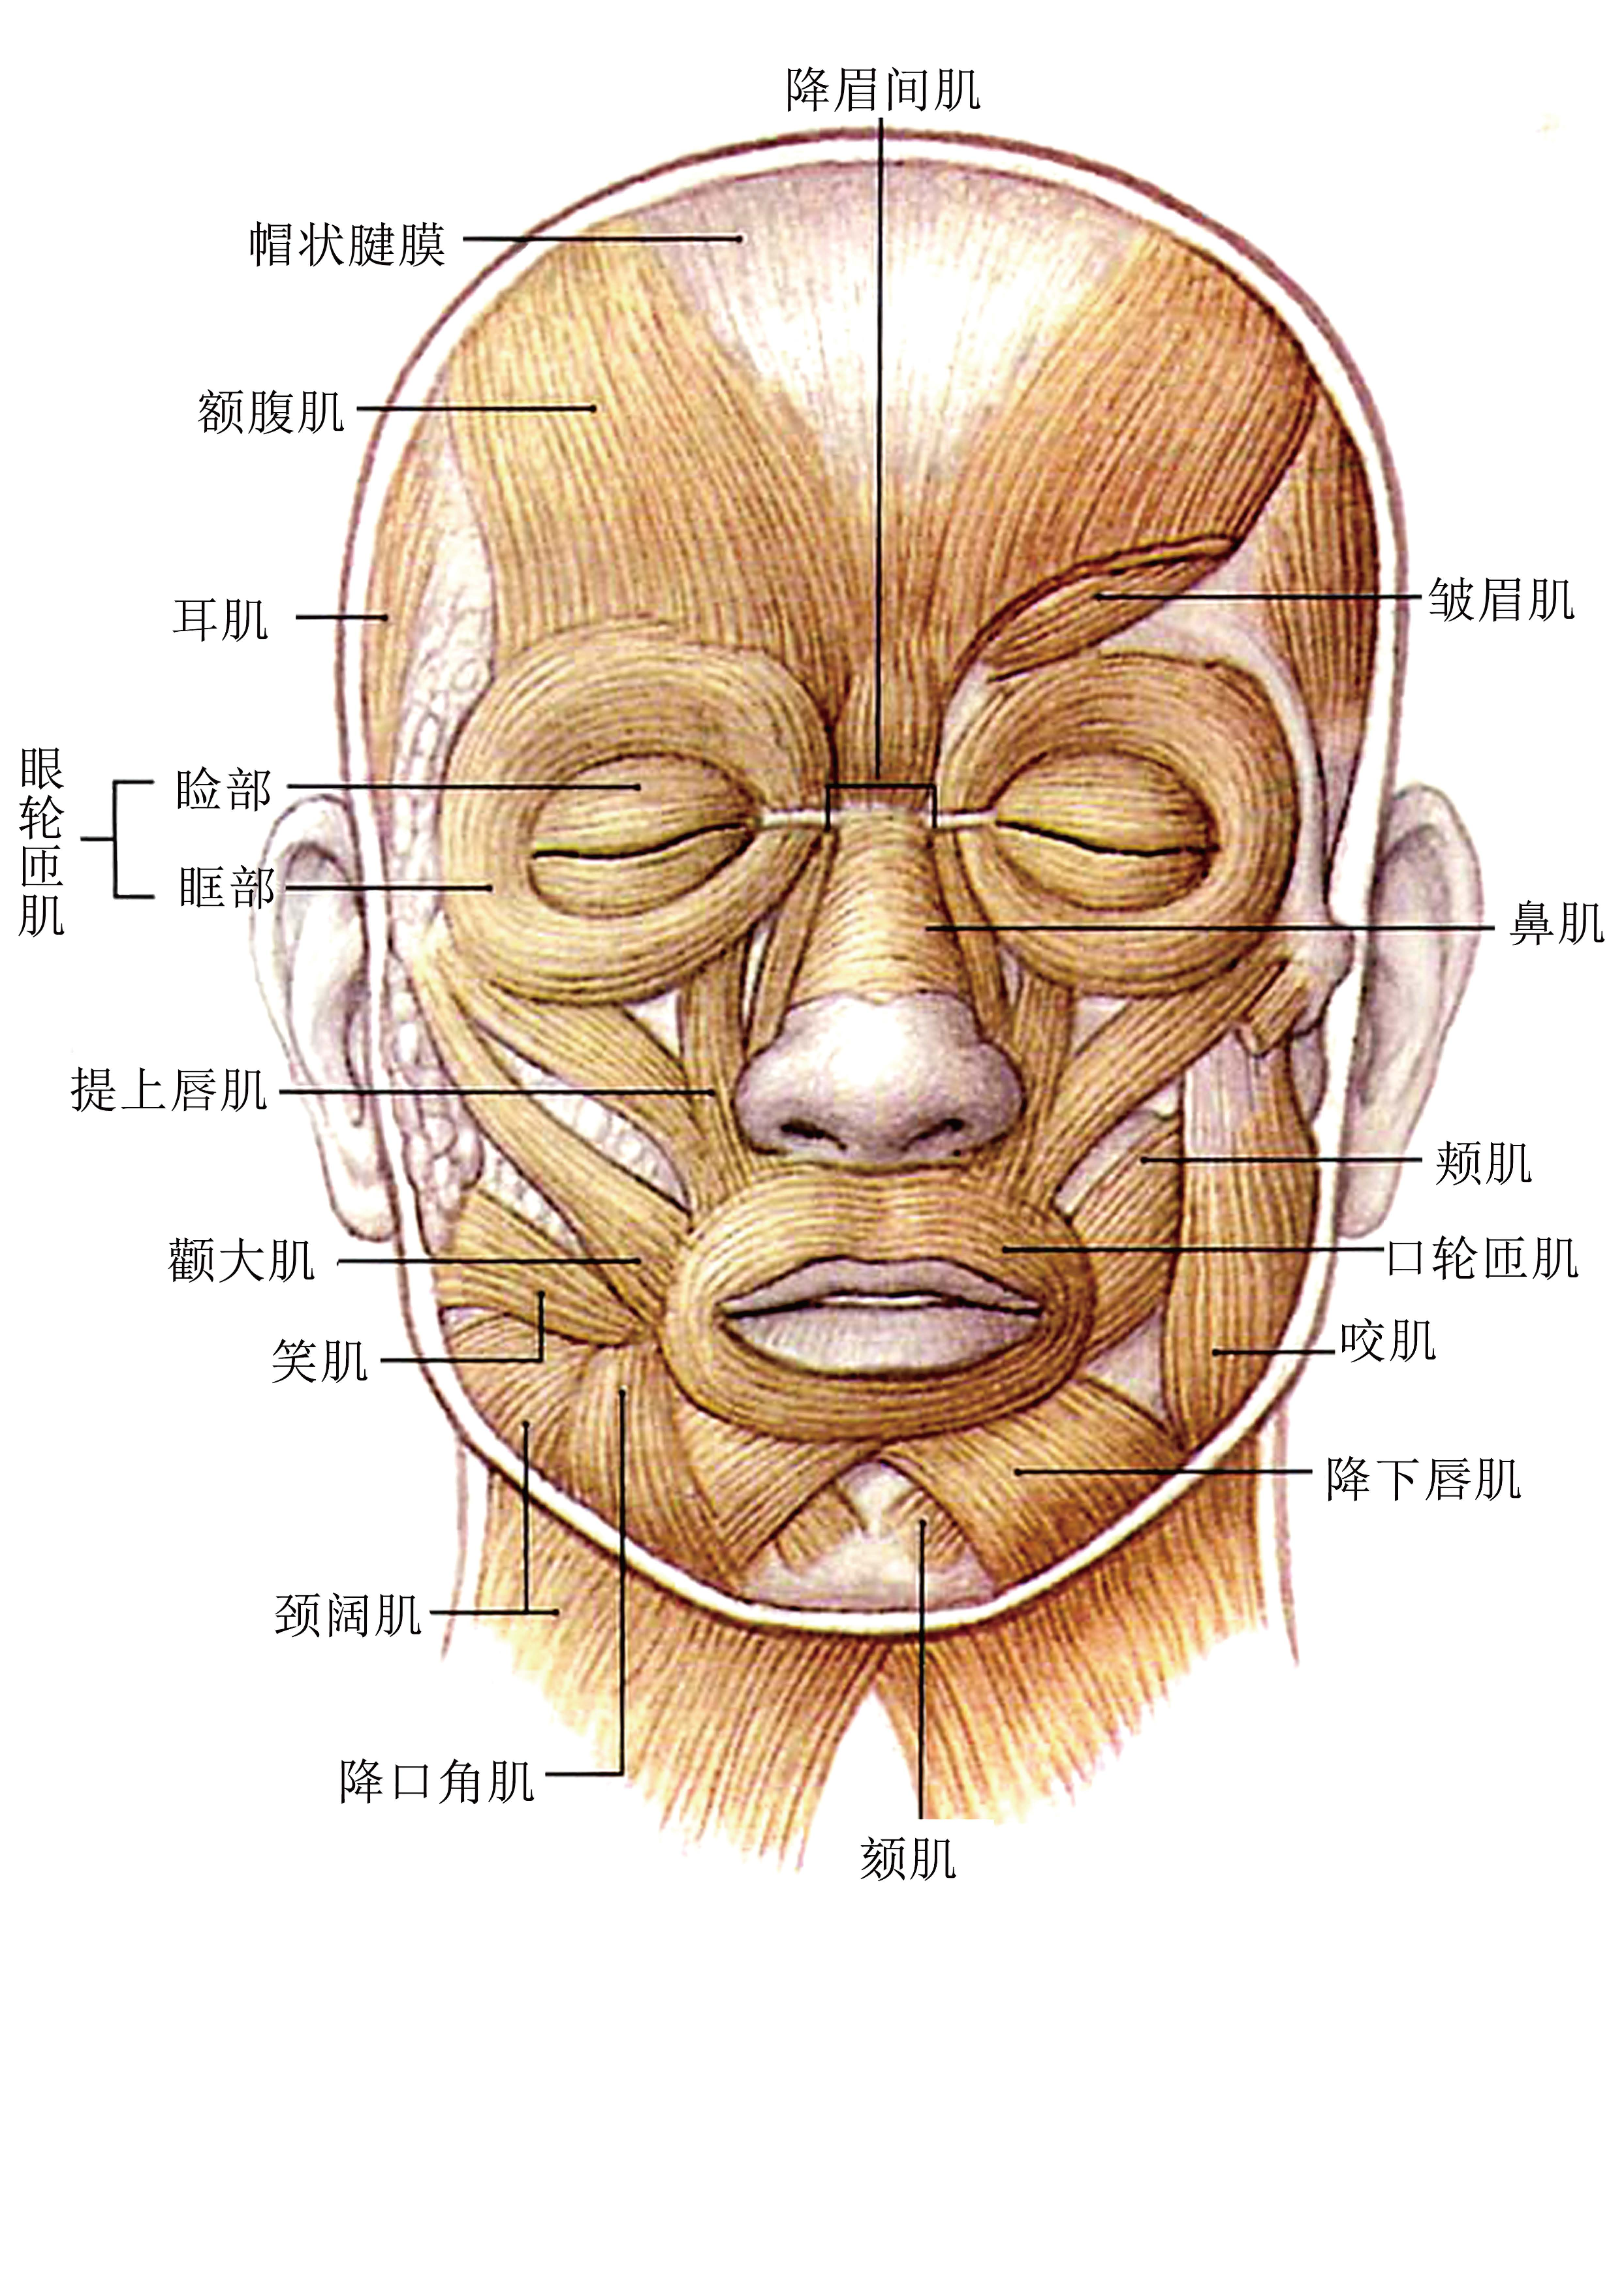
\includegraphics[width=0.28\textwidth]{ME2}
    \caption{人脸面部表情肌肉划分}
    \label{fig4}
\end{figure}

目前存在的宏表情和微表情数据集种类繁多且各具特色,但因为各类研究目的的差异,各类数据集间的迁移效果并不显著,存在着很大的局限性和个体差异性,存在的问题集中表现为以下几点:

首先,各个数据集建立标准不统一。对于常用的宏表情数据集,例如JAFFE和CK+两个宏表情数据集,他们在情感分类的标准上存在差异,JAFFE数据集将表情分为快乐、愤怒、厌恶、讨厌、惊讶、压抑和中性七类,而CK+数据集则在此基础上加入了轻蔑。同样与微表情数据集的分类方式也不一样,例如SMIC微表情数据集将表情分类为积极、消极和惊讶三类,CASME系列数据集将表情分类高兴、惊讶、悲伤、厌恶、恐惧、压抑和其他七种类型。另一方面,对于微表情数据集,不同的数据集之间诱发方式可能也存在差异,例如有的数据集使用自然诱发(SMIC、CASME),有的使用非自然状态下的模拟方式(USF-HD、Polikovsky)。此外差异性还表现在SMIC数据集没有对AU单元进行标注、CASME数据集的光照条件为。所以不同的数据库建立标准导致了难以使用统一的方法对数据集进行性能的评价。

其次,样本数量有限。目前各个数据集的样本数量较少,尤其是参与者的数量有限,这使得某些微表情现象不具有普遍意义,同时也难以提出较强的可说服性理论。

\section{微表情特征提取的一般方法}

\subsection{基于纹理信息的LBP-TOP特征提取符}

局部二值模式(Local Binary Pattern,LBP)是一种用来描述图像局部纹理特征的运算符,它具有旋转不变性和灰度不变性等显著的优点,在人脸识别方面被广泛应
用\citep{Ojala2002Gray}。简单来说,就是对图像中的某一像素点的灰度值与其邻域的像素点的灰度值做比较,如果邻域像素值比该点大,则赋为1,反之,则赋为0。
从图像的左上角开始,形成一个LBP编码,然后将该编码转换为一个十进制数。通过这种转换,可以将一个像素点与邻域的差值关系用一个数表示。

因为LBP特征记录的是像素点与邻域像素的差值关系,所以光照变化只会引起像素值的同增或同减,不会改变LBP值的大小,特别是在局部区域,所以LBP可以很好的保存图
像中像素值的差值关系(如图~\ref{fig5}所示)。进一步的将LBP做直方图统计,这个直方图就可以用来作为纹理分析的特征算子。

\begin{figure}[!htbp]
    \centering
    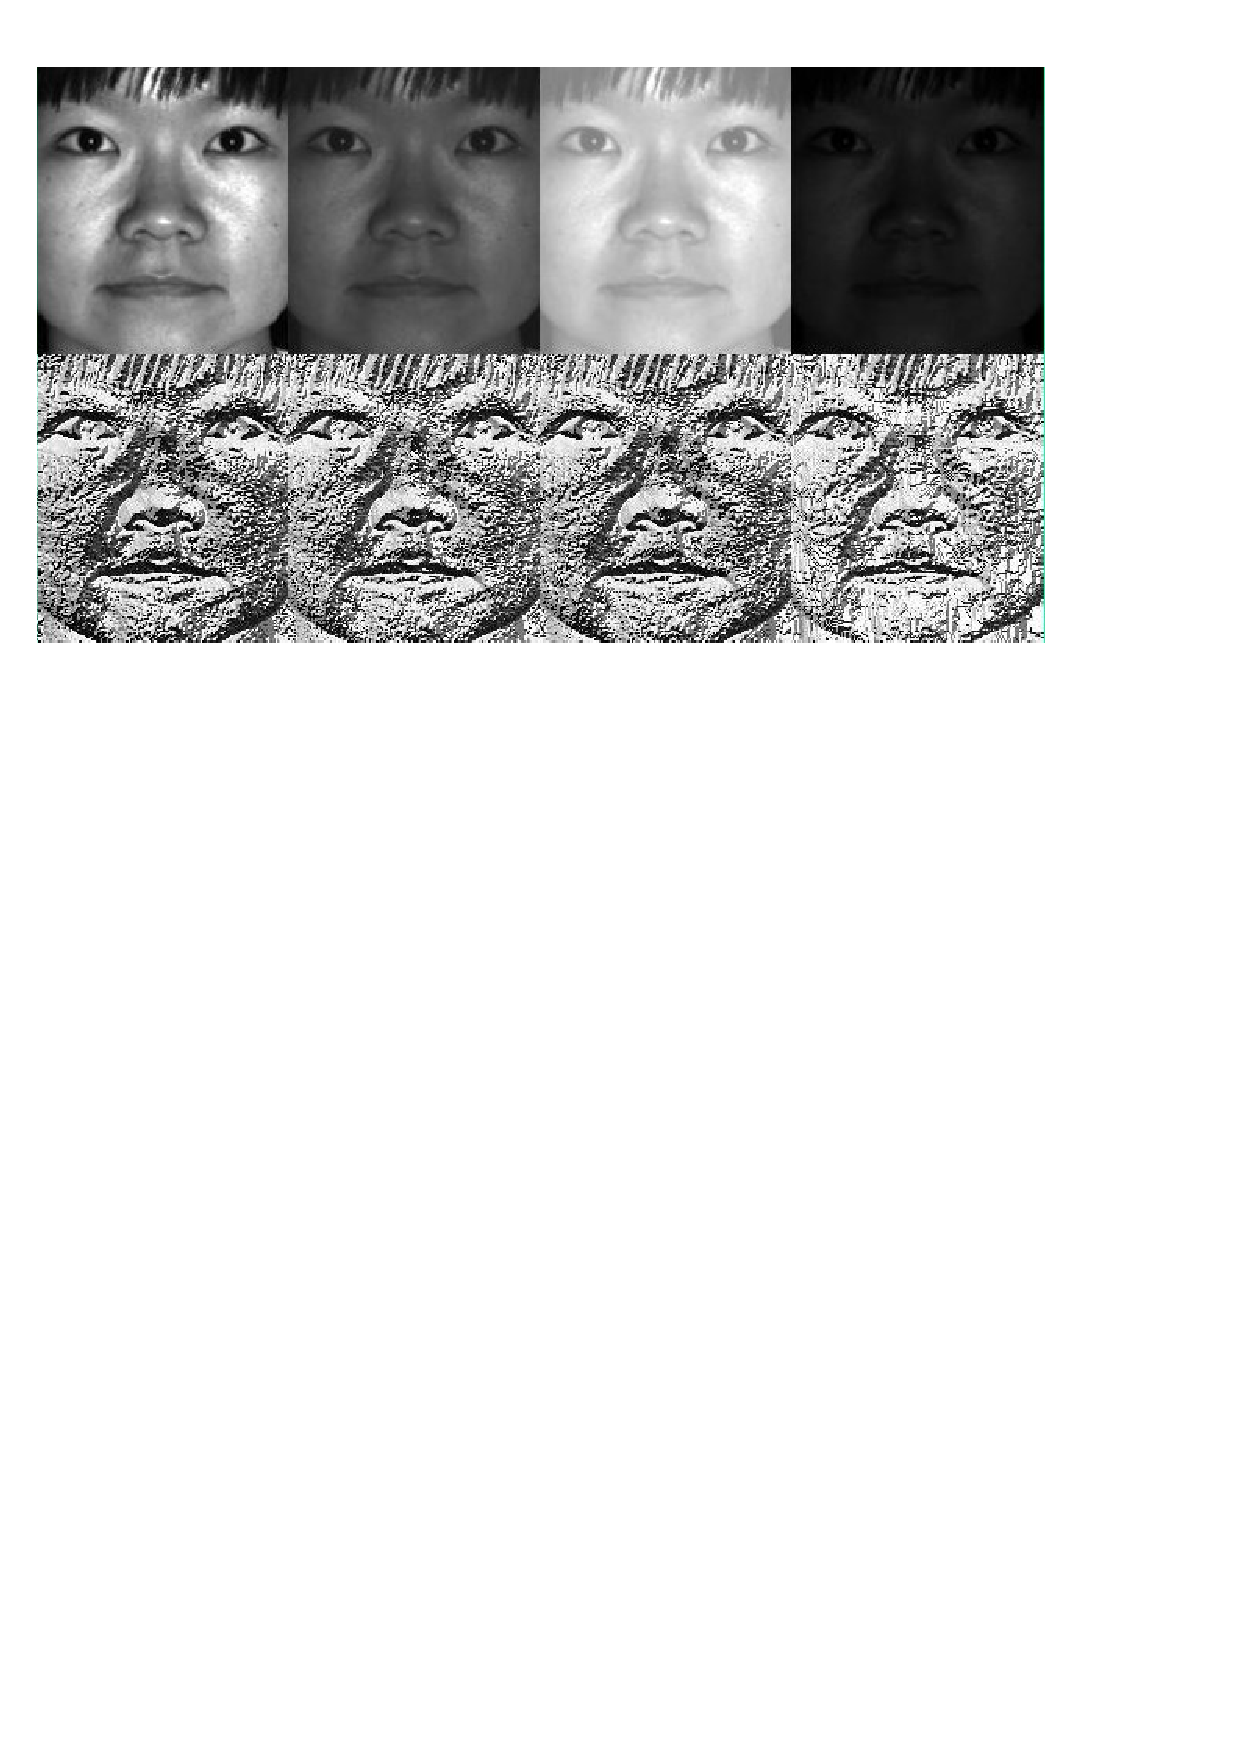
\includegraphics[width=0.5\textwidth]{LBP0}
    \caption{LBP特征的光照鲁棒性}
    \label{fig5}
\end{figure}

但是LBP只能处理单张的二维图像,对于视频或者图像序列则无能为力,2007年芬兰奥卢大学的Zhao等人提出了一种处理动态纹理的LBP特征提取符LBP-TOP,但是现在已经
被广泛用于基于视频的人脸表情识别\citep{zhao2007dynamic}。

LBP-TOP是LBP从二维空间到三维空间的拓展,是在二维图像的X、Y方向上增加了一个沿着时间方向的T轴,形成了互相正交的XY、XT和YT三个平面。 以一个图像序列为单位
组成一个立方体,对其划分合适的块参数(Blocksize),将一个小块作为一个小单元从三个不同的平面提取LBP特征生成该平面的特征直方图,将三个直方图级联为一个基
于块的直方图,以同样的方式遍历整个图像序列立方体,生成最终的LBP-TOP特征直方图,如图~\ref{fig6}所示,中间的三列直方图是小单元的LBP-TOP特征直方图,右侧的直方图是整个立方体的LBP-TOP特征直方图,关于Blocksize的划分将在章节\ref{chap:owner1}中讨论。

\begin{figure}[!htbp]
    \centering
    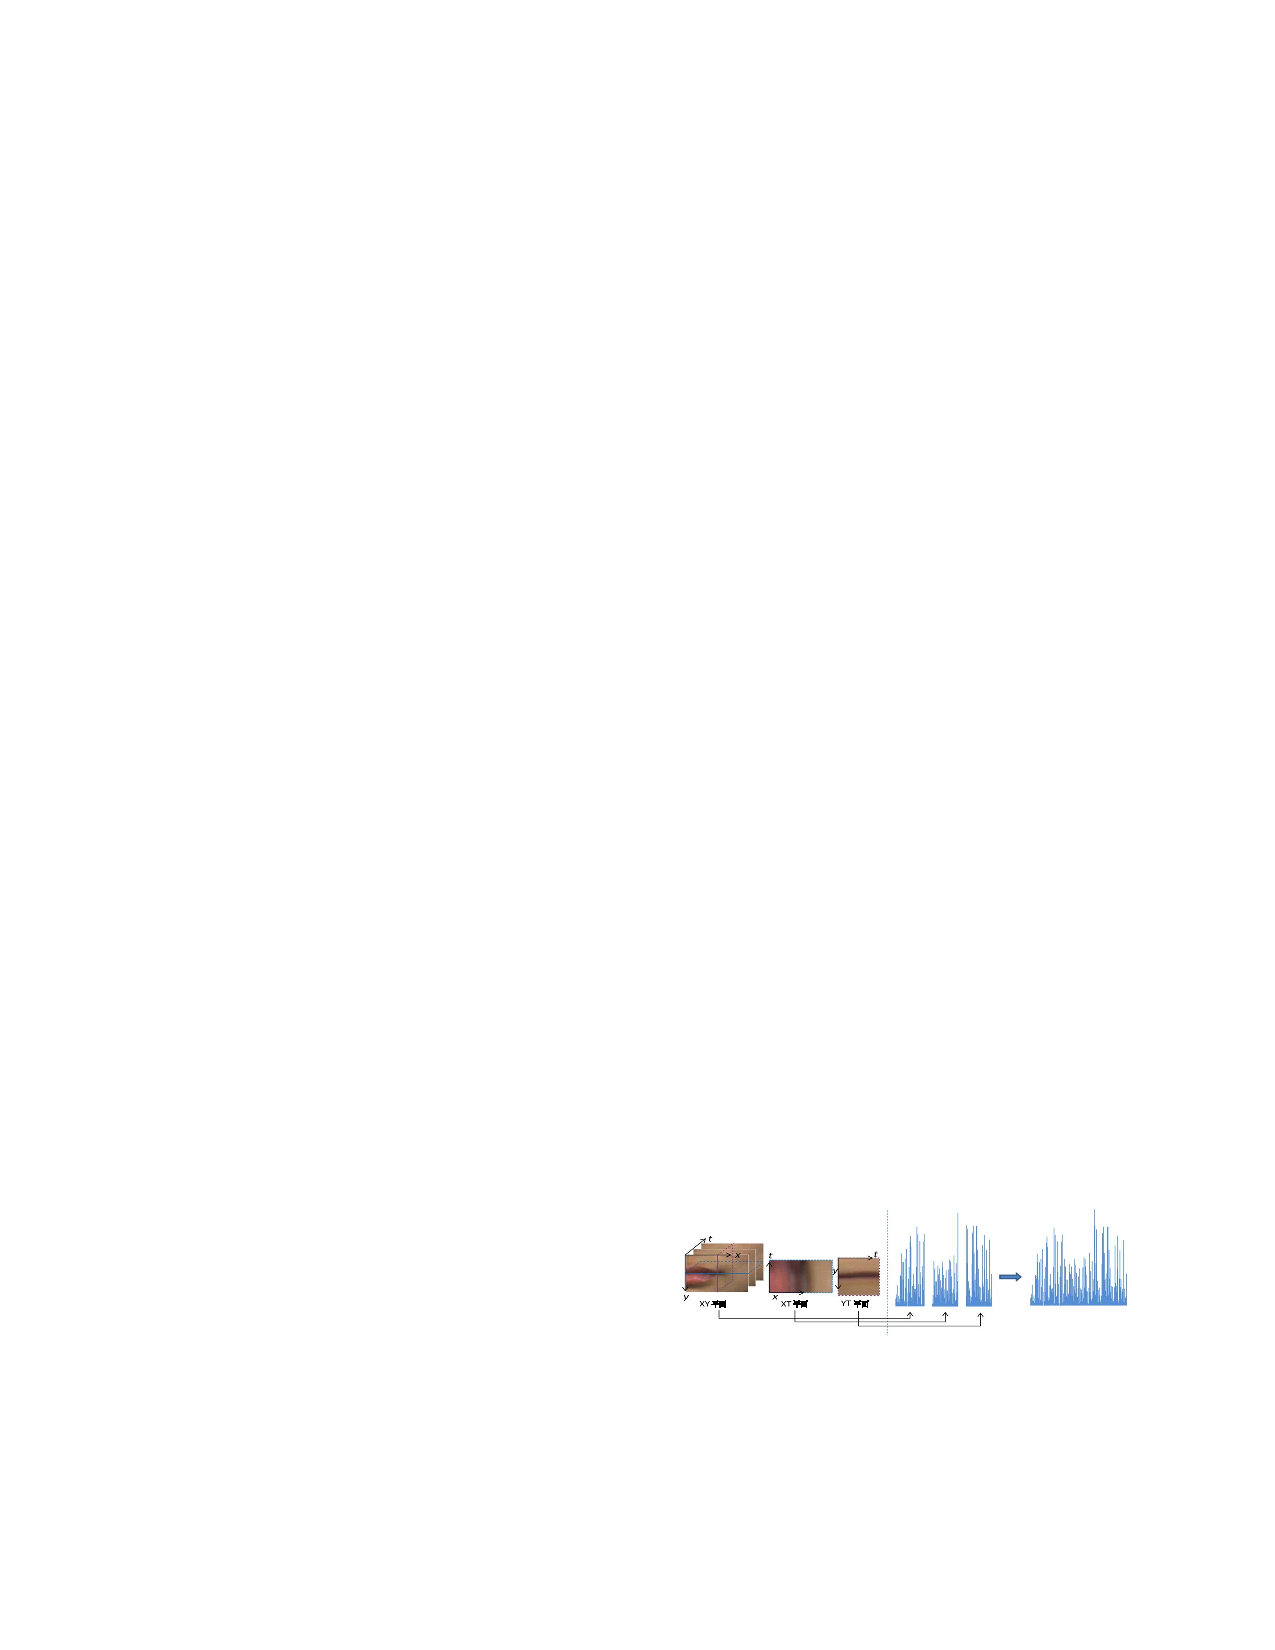
\includegraphics[width=0.9\textwidth]{LBP}
    \caption{LBP-TOP特征提取过程}
    \label{fig6}
\end{figure}

\subsection{基于光流法的特征提取}

二十世纪五十年代心理学家Gibson在其著作\citepns{Gibson1950}中首次提出了环境光(Ambient optic)、环境光阵(Ambient optic array)、光流(Optic flow)和光流阵(Optic flow array)等基本概念。随后,一系列关于昆虫视觉机理方面的实验结果表明,大多数昆虫都可以通过光流测量自身的运动,进而通过积分获得自身飞行的距离。1976年,Poggio和Reichartdt等人在研究昆虫视觉时提出了关于光流的粗略计算形式\citep{poggio1976visual},1981年Horn和Lucas等人将二维速度场与灰度相联系,引入了光流约束方程,为光流计算做出了奠基性的工作\citep{Lucas1981, HORN1981185}。

光流是空间运动物体在观察成像平面上的像素运动的瞬时速度,是利用图像序列中像素在时间域上的变化以及相邻帧之间的相关性来找到上一帧跟当前帧之间存在的对应关系,从而计算出相邻帧之间物体的运动信息的一种方法。一般而言,光流是由于场景中前景目标本身的移动、相机的运动,或者两者的共同运动所产生的。Barron等人对多种光流计算技术进行了总结,按照理论基础与数学方法的区别把它们分成四种:(1)基于区域或者基于特征的匹配方法;(2)基于频域的方法;(3)基于梯度的方法;(4)基于能量的方法\citep{Barron1992}。光流的研究是利用图像序列中的像素强度数据的时域变化和相关性来确定各自像素位置的“运动”,即研究图像灰度在时间上的变化与景象中物体结构及其运动的关系,将二维图像平面特定坐标点上的灰度瞬时变化率定义为光流矢量。光流场(optical flow field)是运动场在二维图像平面上的投影(运动场,物体在三维真实世界中的运动),是一个二维矢量场,包含的信息是图像中像素点的灰度值发生变化趋势的瞬时速度矢量信息,那通俗的讲就是通过一个图像序列,把每张图像中每个像素的运动速度和运动方向找出来就是光流场。研究光流场的目的就是为了从图像序列中近似计算出不能直接得到的运动场。图~\ref{fig7}提供了光流场中光流的大小和方向的表现。

\begin{figure}[!htbp]
    \centering
    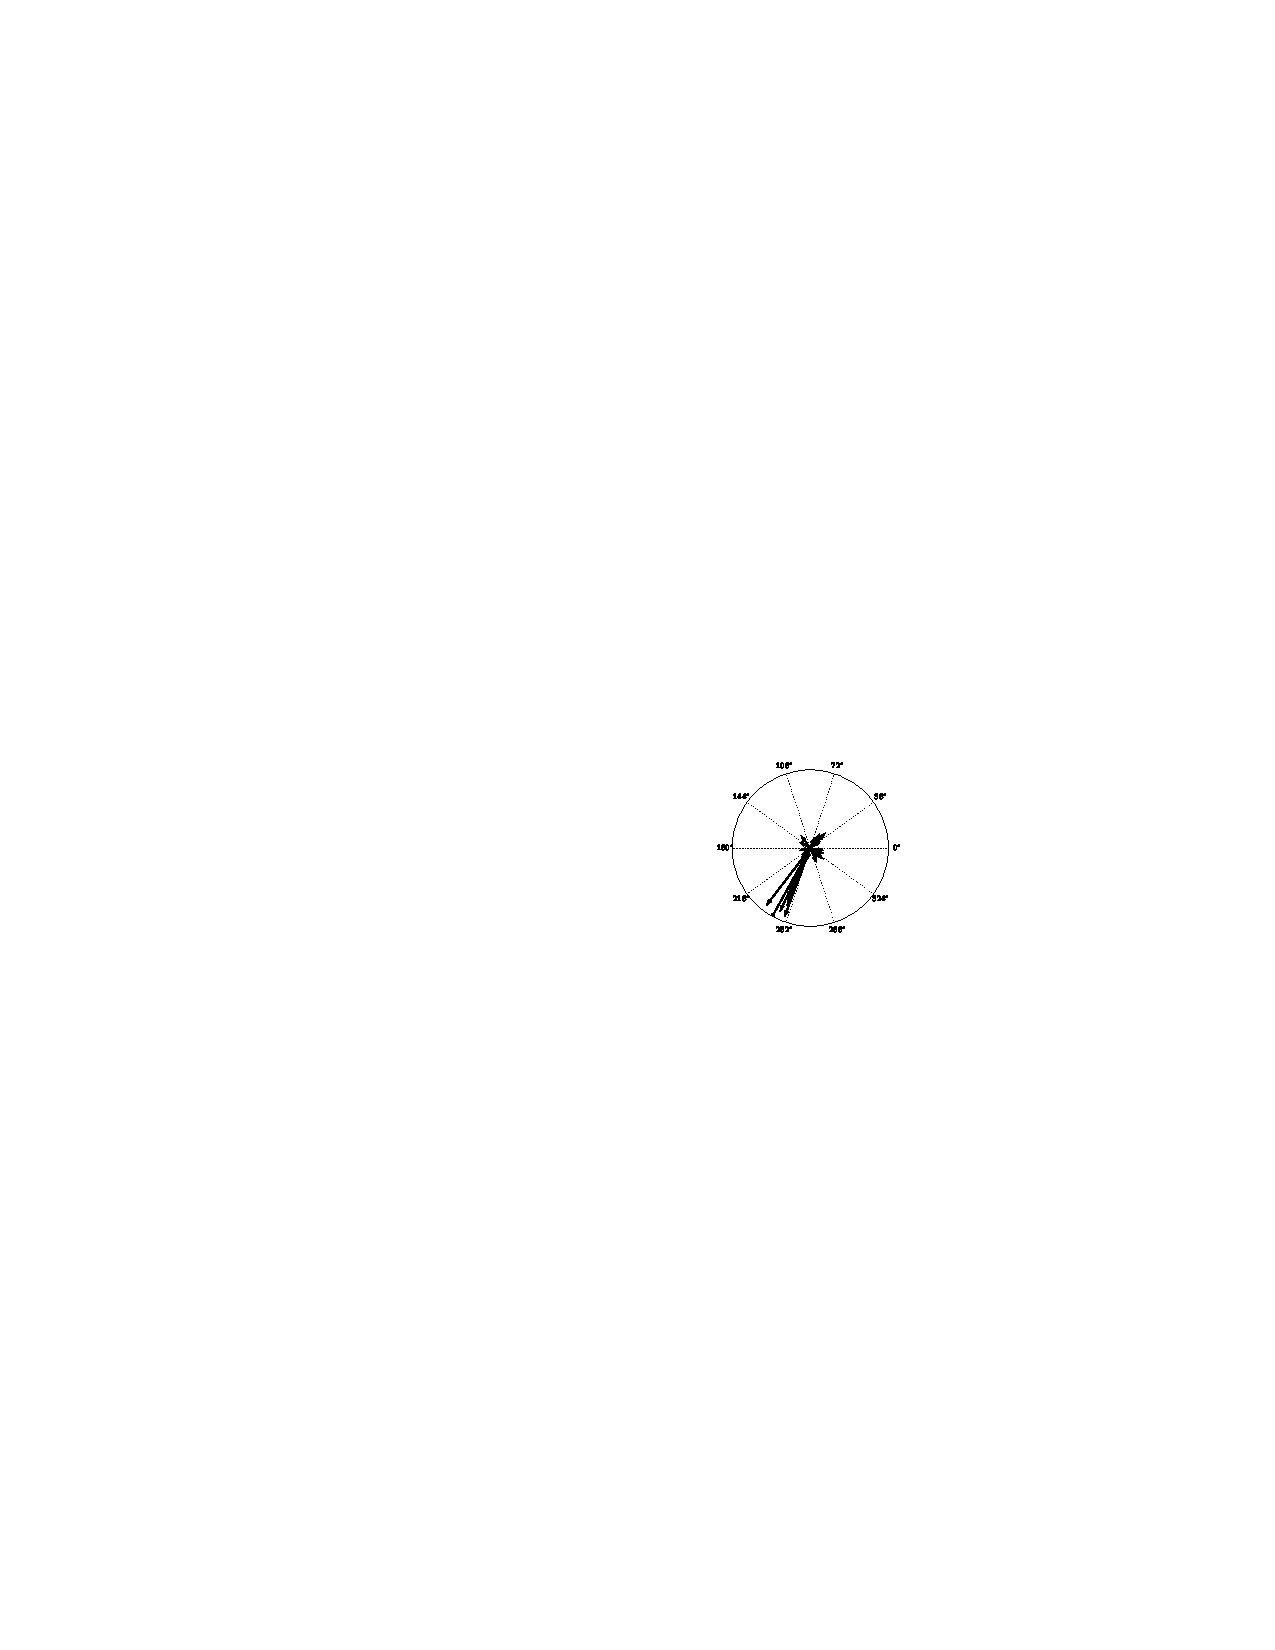
\includegraphics[width=0.30\textwidth]{OF0}
    \caption{光流大小和方向的表现}
    \label{fig7}
\end{figure}

光流法检测运动目标,其基本思想是赋予图像中的每一个像素点一个速度矢量,从而形成了该图像的运动场。图像上的点和三维物体上的点在某一特定的运动时刻是一一对应的,根据各像素点的速度矢量特征对图像进行动态的分析。若图像中不存在运动目标,那么光流矢量在整个图像区域则是连续变化的,而当物体和图像背景中存在相对运动时,运动物体所形成的速度矢量则必然不同于邻域背景的速度矢量,从而将运动物体的位置检测出来。但光流法的计算过于复杂,而且在实际情况中由于各种复杂的环境因素常常会导致计算结果出现很大的误差,故对它的使用必须是在建立一定前提假设的基础之上的:(1)相邻帧之间保持亮度恒定不变;(2)相邻帧的取帧时间保持连续或物体运动幅度小;(3)具有空间一致性,同一子图的像素点具有相同的运动。

光流不能由运动图像的局部信息来唯一的确定,例如,亮度等值线上的点或者亮度比较均匀的区域都无法唯一的确定其点的运动对应性,但是运动是可以进行观察得到。当人的眼睛观察运动物体时,物体的景象在人眼的视网膜上形成一系列连续变化的图像,这一系列连续变化的信息不断“流过”视网膜(即图像平面),由于它包含了目标运动的信息,因此可被观察者用来确定目标的运动情况。由此说明运动场和光流不一定是唯一对应的,即光流不一定是由物体运动产生的,反之如果物体发生了运动也不一定就能产生光流。但是一般情况下,表观运动和物体真实运动之间的差异是可以忽略的,可以用光流场代替运动场来分析图像中的运动目标及其相关的运动参数。

\subsection{基于Gabor的特征提取}

% Gabor特征是一种可以用来描述图像纹理信息的特征,Gabor滤波器的频率和方向与人类的视觉系统类似,特别适合于纹理表示与判别。Gabor特征主要依靠Gabor核在频率域上对信号进行加窗,从而能描述信号的局部频率信息。
% 说到Gabor核,不能不提到傅里叶变换。正是靠傅里叶变换,我们才能将信号转换到频率域,才能让Gabor核在频率域去加窗。而在原本的空间域中,一个Gabor核实际上就是一个高斯核与正弦波调制的结果,可以看做是高斯核应用在了正弦波的频域部分。
% 先对图像I(x,y)进行实数形式的Gabor变换,得到处理后的图像,直接提取特征的话,特征维数太高,不利于后续处理。一般对图像分块,然后计算每一块对应的能量。

Gabor小波与人类视觉系统中简单细胞的视觉刺激响应非常相似,它在提取目标的局部空间和频率域信息方面具有良好的特性\citep{Daugman1988,Kyrki2004Simple}。虽然Gabor小波本身并不能构成正交基,但在特定参数下可构成紧框架。Gabor小波对于图像的边缘敏感,能够提供良好的方向选择和尺度选择特性,而且对于光照变化不敏感,能够提供对光照变化良好的适应性。上述特点使Gabor小波被广泛应用于视觉信息理解。二维Gabor小波变换是在时频域进行信号分析处理的重要工具,其变换系数有着良好的视觉特性和生物学背景,因此被广泛应用于图像处理、模式识别等领域。与传统的傅立叶变换相比,Gabor小波变换具有良好的时频局部化特性。即非常容易地调整Gabor滤波器的方向、基频带宽及中心频率从而能够最好的兼顾信号在时空域和频域中的分辨能力;Gabor小波变换具有多分辨率特性即变焦能力。即采用多通道滤波技术,将一组具有不同时频域特性的Gabor小波应用于图像变换,每个通道都能够得到输入图像的某种局部特性,这样可以根据需要在不同粗细粒度上分析图像。此外,在特征提取方面,Gabor小波变换与其它方法相比:一方面其处理的数据量较少,能满足系统的实时性要求;另一方面,小波变换对光照变化不敏感,且能容忍一定程度的图像旋转和变形,当采用基于欧氏距离进行识别时,特征模式与待测特征不需要严格的对应,故能提高系统的鲁棒性。

无论从生物学的角度还是技术的角度,Gabor特征都有很大的优越性。研究表明,在基本视觉皮层里的简单细胞的感受野局限在很小的空域范围内,并且高度结构化。Gabor变换所采用的核与哺乳动物视觉皮层简单细胞2D感受野剖面非常相似,具有优良的空间局部性和方向选择性,能够抓住图像局部区域内多个方向的空间频率(尺度)和局部性结构特征。这样,Gabor分解可以看作一个对方向和尺度敏感的有方向性的显微镜。同时,二维Gabor函数也类似于增强边缘以及峰、谷、脊轮廓等底层图像特征,这相当于增强了被认为是面部关键部件的眼睛、鼻子、嘴巴等信息,同时也增强了诸于黑痣、酒窝、伤疤等局部特征,从而使得在保留总体人脸信息的同时增强局部特性成为可能.它的小波特性说明了Gabor滤波结果是描述图像局部灰度分布的有力工具,因此,可以使用Gabor滤波来抽取图像的纹理信息. 由于Gabor特征具有良好的空间局部性和方向选择性,而且对光照、姿态具有一定的鲁棒性,因此在人脸识别中获得了成功的应用。然而,大部分基于Gabor特征的人脸识别算法中,只应用了Gabor幅值信息,而没有应用相位信息,主要原因是Gabor相位信息随着空间位置呈周期性变化,而幅值的变化相对平滑而稳定,幅值反映了图像的能量谱,Gabor幅值特征通常称为Gabor能量特征(Gabor energy features)。Gabor小波可像放大镜一样放大灰度的变化,人脸的一些关键功能区域(眼睛、鼻子、嘴、眉毛等)的局部特征被强化,从而有利于区分不同的人脸图像。Gabor小波核函数具有与哺育动物大脑皮层简单细胞的二维反射区相同的特性,即具有较强的空间位置和方向选择性,并且能够捕捉对应于空间和频率的局部结构信息;Gabor滤波器对于图像的亮度和对比度变化以及人脸姿态变化具有较强的健壮性,并且它表达的是对人脸识别最为有用的局部特征。Gabor小波是对高级脊椎动物视觉皮层中的神经元的良好逼近,是时域和频域精确度的一种折中。

通过上面的分析,我们知道一个Gabor核能获取到图像某个频率邻域的响应情况,这个响应结果可以看做是图像的一个特征。那么,我们如果用多个不同频率的Gabor核去获取图像在不同频率邻域的响应情况,最后就能形成图像在各个频率段的特征,这个特征就可以描述图像的频率信息了,由于纹理特征通常和频率相关,因此Gabor核经常用来作为纹理特征。

\section{相关深度学习网络}

深度学习方法作为机器学习尤其是神经网络方法的一种,在图像处理、视频分析和语音识别等领域产生了许多成功的案例。端到端的神经网络模型能够通过学习大量高维数据进行分类和预测,这减少了人工特征工程的繁杂操作。卷积神经网络作为应用最广泛的深度学习方法之一,目前在很多图像相关领域都处于无可替代的地位。卷积神经网络最早出现在论文\citepns{lecun1998gradient}的研究中,在过去的几年里,卷积神经网络经过了大量的分层、分块等设计的修改,诞生了许多成功的衍生网络如AlexNet\citep{krizhevsky2012imagenet}、VGG-Net\citep{Simonyan2014Very}和GoogLeNet\citep{szegedy2015going}等。最近,有很多将深度学习应用于微表情识别的研究,然而,由于是在小数据集上使用的深度网络,所获得的识别准确度仅在随机水平左右。

\subsection{三维卷积神经网络}

二维卷积神经网络被认为是解决图像识别问题的一种强大的模型,但将二维卷积神经网络应用到视频中却并非易事,在视频中应用二维卷积神经网络一个简单的方法就是对每一帧运用卷积来识别,但是这种方法并没有考虑到连续帧间的时间维度信息。一些研究表明,三维卷积能够从空间和时间两个维度提取特征,从而获取多个相邻帧中编码的运动信息。三维卷积神经网络从输入帧中生成多个通道的信息,并结合所有通道的信息得到最终的特征表示。该方法应用到现实环境中的人类行为识别中,在不依赖于人工提取的特性的情况下取得了优异的性能\citep{Shuiwang20133D}。

三维卷积是通过将一个三维核与叠加在一起的多个连续帧形成的立方体进行卷积来实现的。在这个结构中,卷积层中每一个特征映射都会与前一层中多个相邻的连续帧相连,从而获取运动信息。需要注意的是:三维卷积核只能从立方体中提取一类特征,因为在整个立方体中卷积核的权值都是一样的,也就是共享权值。所以我们可以采用多种卷积核,以提取多种特征。对于卷积神经网络有一个通用的设计规则,在后面的层(离输出层近的)特征映射的个数应该增加,这样就可以从低级的特征映射组合产生更多类型的特征。

\begin{figure}[!htbp]
    \centering
    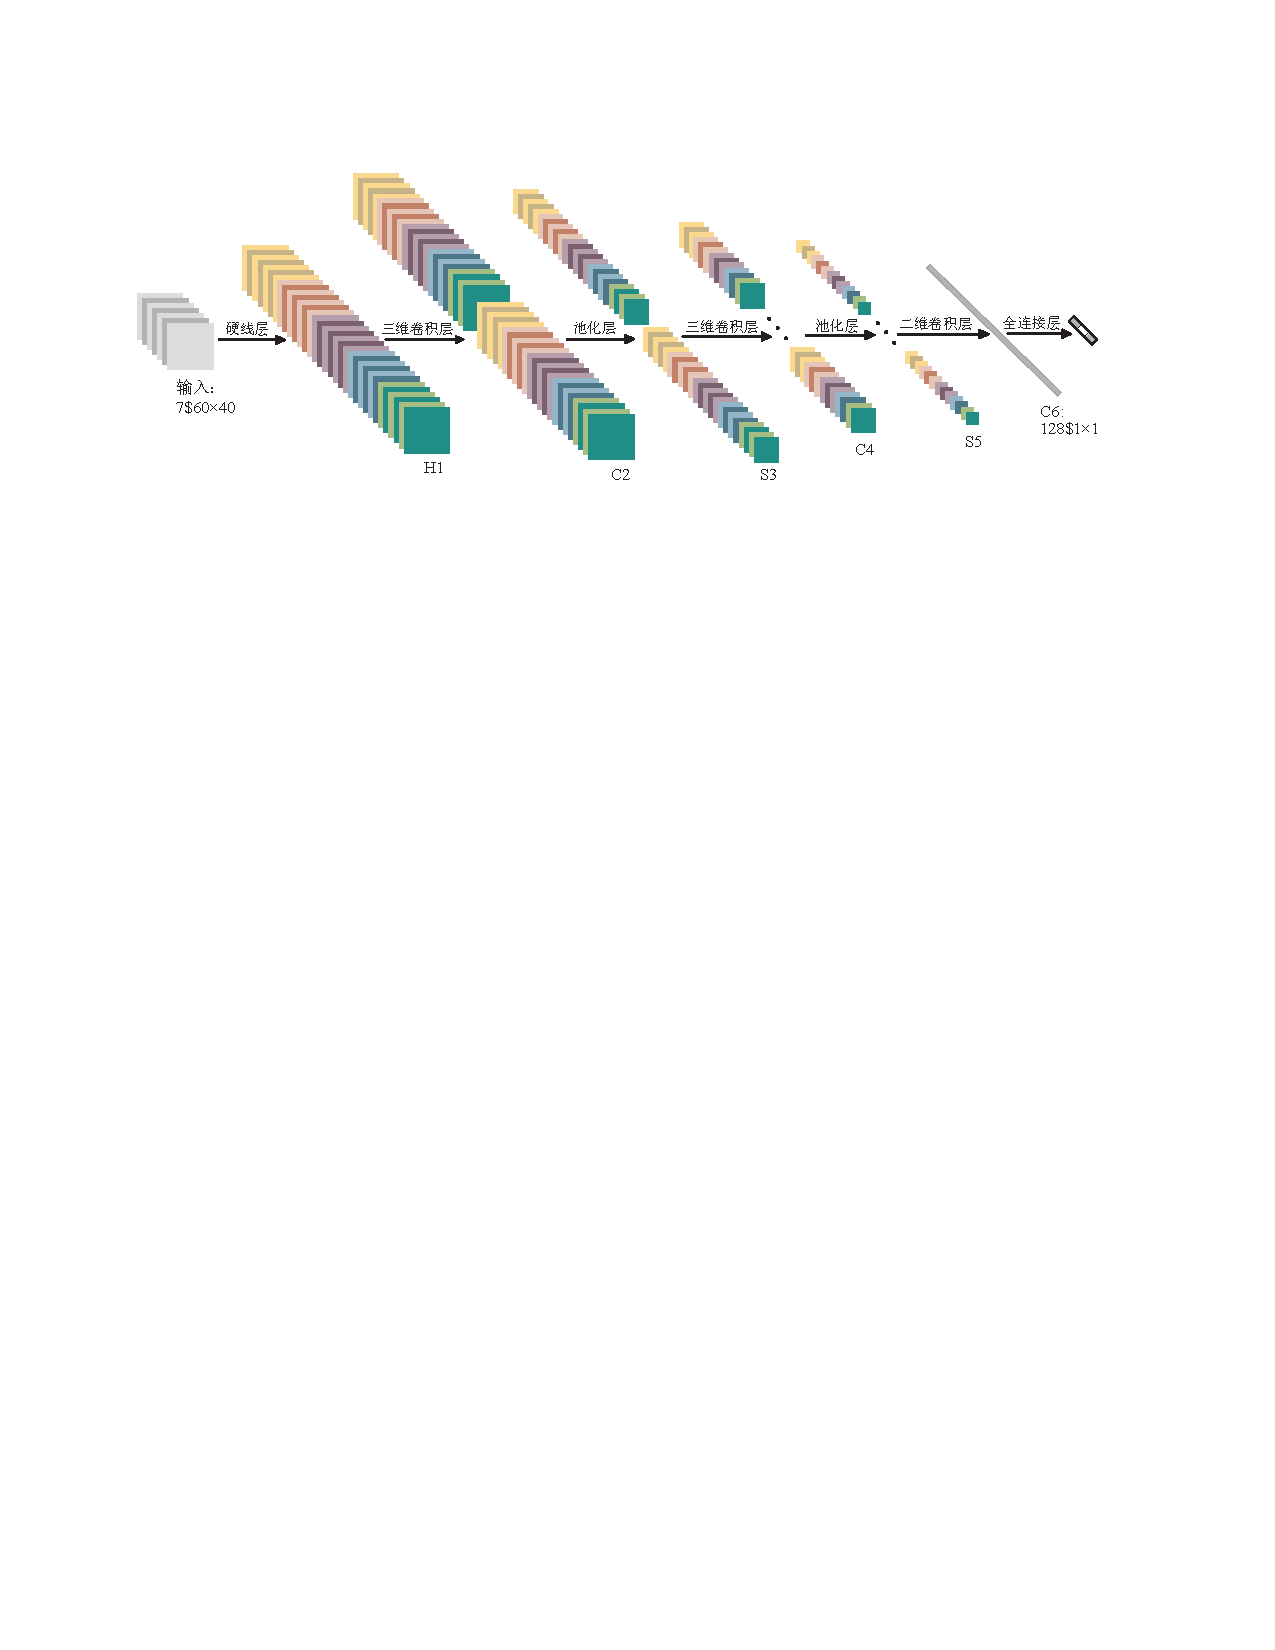
\includegraphics[width=0.95\textwidth]{3DCNN1}
    \caption{三维卷积神经网络架构}
    \label{fig8}
\end{figure}

如图~\ref{fig8}所示,该架构包含一个硬线层、三个卷积层、两个池化层和一个全连接层。每个三维卷积核卷积的立方体是连续的七帧,每帧块大小为$60\times40$;第一层应用了一个固定的硬线核去对原始的帧进行处理,产生多个通道的信息,然后对多个通道分别处理。最后再将所有通道的信息组合起来得到最终的特征描述。

H1为硬线层(Hardwired),每帧提取五个通道的信息,分别是灰度、$x$和$y$方向的梯度,$x$和$y$方向的光流。其中,前面三个都可以每帧都计算。然后水平和垂直方向的光流场需要两个连续帧才确定。

C2为卷积层(Convolution),以硬线层的输出作为该层的输入,用一个三维卷积核在五个通道的每一个通道分别进行卷积。同时为了增加特征映射的个数(实际上就是提取不同的特征),在每一个位置都采用两个不同的卷积核。

S3为池化层(Sub-sampling),得到相同数目但是空间分辨率降低的特征映射。

C4为卷积层,对五个通道分别采用三维卷积核,同样,为了增加特征映射个数,在每个位置都采用三种不同的卷积核。

S5为池化层,对每个特征映射采用核进行降采样操作,在这个阶段,每个通道的特征映射都很小。

C6为卷积层,此时对每个特征映射采用二维卷积核进行卷积操作,然后输出为减小到$1×1$大小的特征映射。

经过多层的卷积和下采样后,每连续7帧的输入图像都被转化为一个128维的特征向量,这个特征向量捕捉了输入帧的运动信息。输出层的节点数与行为的类型数目一致,而且每个节点与C6中这128个节点是全连接的。最后,采用一个线性分类器来对这128维的特征向量进行分类,实现行为的识别。

\subsection{残差神经网络}

增加网络的宽度和深度可以很好的提高网络的性能,深的网络一般都比浅的的网络效果好,但对于原来的网络,如果简单地增加深度,会导致梯度弥散或梯度爆炸。对于该问题的解决方法是正则化初始化和中间的正则化层(Batch Normalization),这样的话可以训练几十层的网络。虽然通过上述方法能够训练,但是又会出现退化问题。在实验中的表现就是虽然网络层数增加,但在训练集上的准确率却饱和甚至下降了(这个不能简单的解释为过拟合现象,因为过拟合时应该在训练集上表现的更好)。通过浅层网络等同映射构造深层模型,结果深层模型并没有比浅层网络有等同或更低的错误率,推断退化问题可能是因为深层的网络并不是那么好训练,也就是求解器很难去利用多层网络拟合同等函数。

针对这个问题He等在2015年提出了一种全新的网络,叫深度残差神经网络(Deep residual neural network),它允许网络尽可能的加深,其中引入了全新的结构,如图~\ref{fig9}所示\citep{he2016deep}。

\begin{figure}[!htbp]
    \centering
    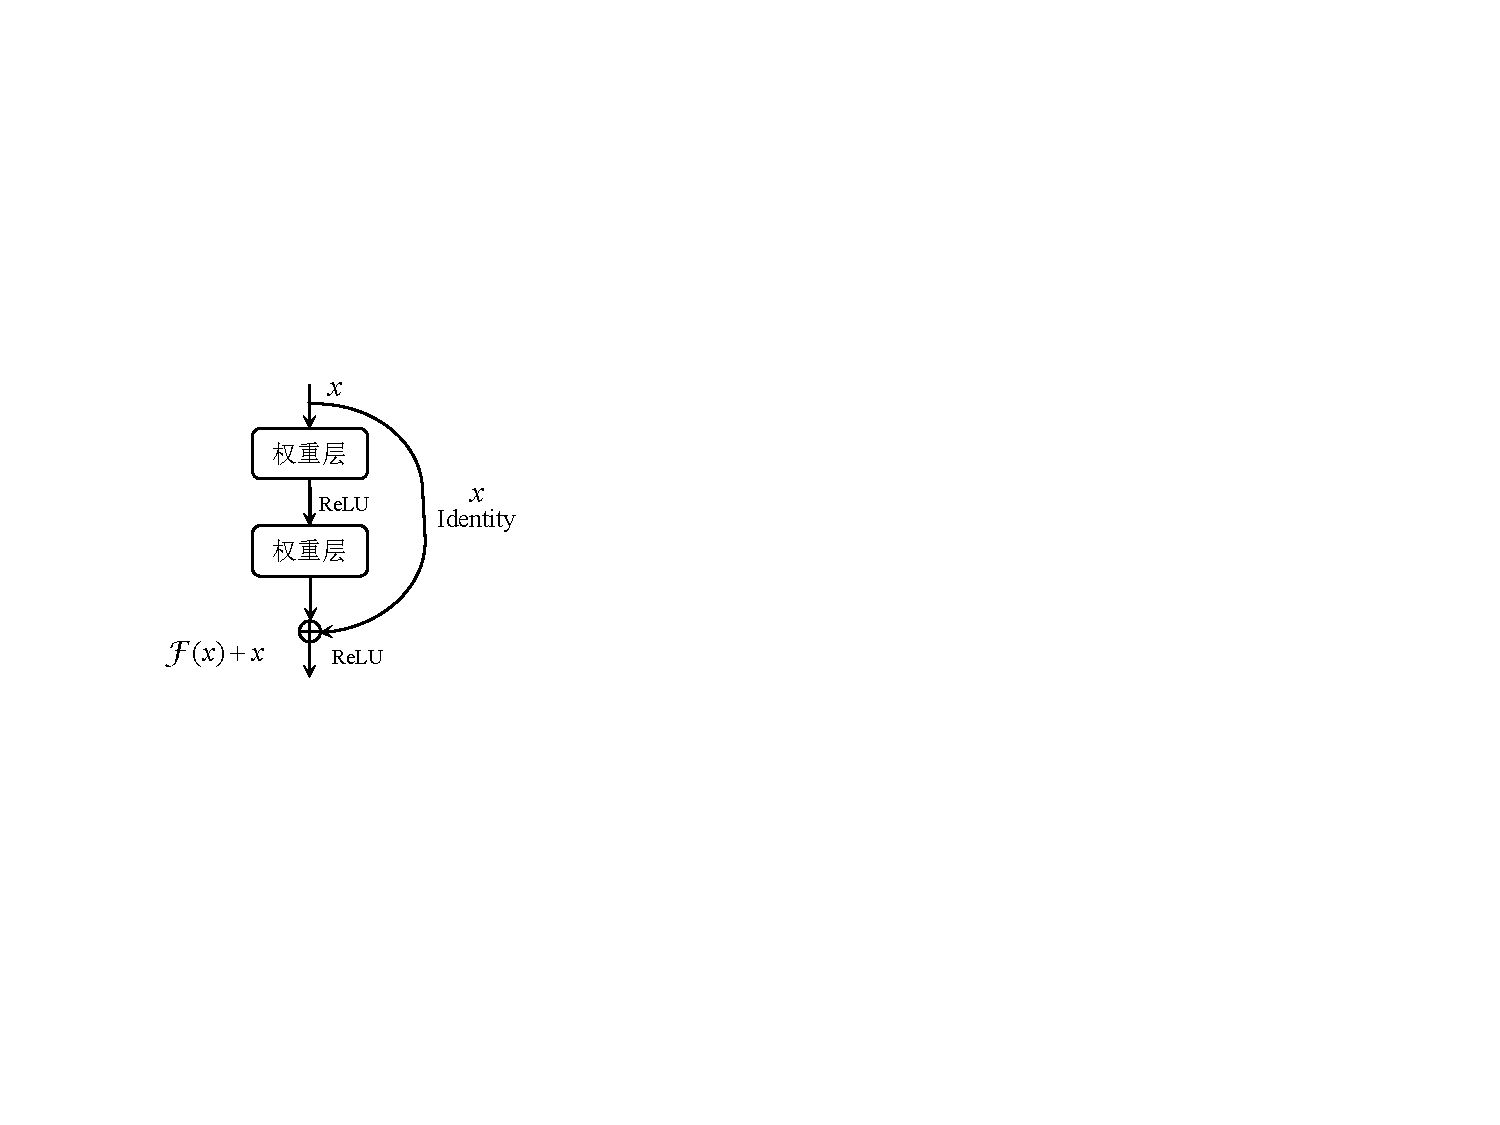
\includegraphics[width=0.40\textwidth]{RESNET0}
    \caption{ResNet的残差学习模块}
    \label{fig9}
\end{figure}

理论上,对于“随着网络加深,准确率下降”的问题,ResNet提出了两种Mapping:一种是Identity mapping,指图~\ref{fig9}中的弧线,另一种是Residual mapping,指除了弧线以外的部分,所以最后的输出是$y=\mathcal{F}\left ( x \right )+x$ 。Identity mapping指自身,也就是公式中的$x$ ,而Residual mapping指的是“差”,也就是$y-x$ ,所以残差指的就是$\mathcal{F}\left (x \right )$部分。如果网络已经到达最优,继续加深网络,Residual mapping将被转化为0,只剩下Iidentity mapping,这样理论上网络一直处于最优状态了,网络的性能也就不会随着深度增加而降低了。

由上可以看出残差网络t的主要思想是在网络中增加了直连通道,即Highway network的思想,它允许原始输入信息直接传到后面的层中\citep{Srivastava2015Highway},这样的话这一层的神经网络可以不用学习整个的输出,而是学习上一个网络输出的残差。

% 残差网络以前在不增加网络复杂性的情况下,在基于图像的识别任务上实现了最优性能。残差网络通常使用残差块来构建网络,而典型的残差块如图~\ref{fig9}所示。在残差块中,将添加一个捷径来执行标识映射(通过元素汇总实现),这有助于减少退化问题。捷径还加快了训练过程,几乎不引入额外的参数和计算。

传统的卷积网络或者全连接网络在信息传递的时候或多或少会存在信息丢失、损耗等问题,同时还会导致梯度弥散或梯度爆炸,导致很深的网络无法训练。残差网络在一定程度上解决了这个问题,通过直接将输入信息绕道传到输出,保护信息的完整性,整个网络只需要学习输入、输出差别的那一部分,简化学习目标和难度。残差网络的结构可以极快的加速神经网络的训练,模型的准确率也有比较大的提升。残差网络在ImageNet比赛分类任务上获得第一名,因为它“简单与实用”并存,之后很多方法都建立在ResNet50或者ResNet101的基础上完成,检测、分割、识别等领域都纷纷使用残差网络,Alpha zero也使用了残差网络,所以可见残差网络确实很好用。
